%%% One-side print:
\documentclass[11pt,a4paper]{report}
\usepackage[top=25mm,bottom=25mm,right=25mm,left=30mm,head=12.5mm,foot=12.5mm]{geometry}
\let\openright=\clearpage

%%% Two-side print:
%\documentclass[11pt,a4paper,twoside,openright]{report}
%\usepackage[top=25mm,bottom=25mm,right=25mm,left=30mm,head=12.5mm,foot=12.5mm]{geometry}
%\let\openright=\cleardoublepage

%%% Definition of some useful macros
%%% Tento soubor obsahuje definice různých užitečných maker a prostředí %%%
%%% Další makra připisujte sem, ať nepřekáží v ostatních souborech.     %%%
%%% This file contains definitions of various useful macros and environments      %%%
%%% Assign additional macros here so that they do not interfere with other files. %%%

\usepackage[a-2u]{pdfx}     % výsledné PDF bude ve standardu PDF/A-2u
                            % resulting PDF will be in the PDF / A-2u standard

\usepackage{ifpdf}
\usepackage{ifxetex}
\usepackage{ifluatex}

%%% Nastavení pro použití samostatné bibliografické databáze.
%%% Settings for using a separate bibliographic database.
\usepackage[
   backend=biber
 ,style=iso-authoryear
  % ,style=iso-numeric
  ,sortlocale=cs_CZ
  ,alldates=iso
  ,bibencoding=UTF8
  ,maxnames=2
  ,maxbibnames=99
  ,block=ragged
]{biblatex}
\let\cite\parencite
\renewcommand*{\multinamedelim}{, \addspace}
\renewcommand*{\finalnamedelim}{\addspace a \addspace}

\bibliography{bibliography}

%% Přepneme na českou sazbu, fonty Latin Modern a kódování češtiny
\ifthenelse{\boolean{xetex}\OR\boolean{luatex}}
   { % use fontspec and OpenType fonts with utf8 engines
			\usepackage[english,slovak,czech]{babel}
			\usepackage[autostyle,english=british,czech=quotes]{csquotes}
			\usepackage{fontspec}
			\defaultfontfeatures{Ligatures=TeX,Scale=MatchLowercase}
   }
   {
			\usepackage[english,slovak,czech]{babel}
			\usepackage{lmodern}
			\usepackage[T1]{fontenc}
			\usepackage{textcomp}
			\usepackage[utf8]{inputenc}
			\usepackage[autostyle,english=british,czech=quotes]{csquotes}
	 }
\ifluatex
\makeatletter
\let\pdfstrcmp\pdf@strcmp
\makeatother
\fi

%%% Další užitečné balíčky (jsou součástí běžných distribucí LaTeXu)
\usepackage{amsmath}        % rozšíření pro sazbu matematiky / extension for math typesetting
\usepackage{amsfonts}       % matematické fonty / mathematical fonts
\usepackage{amssymb}        % symboly / symbols
\usepackage{amsthm}         % sazba vět, definic apod. / typesetting of sentences, definitions, etc.
\usepackage{bm}             % tučné symboly (příkaz \bm) / bold symbols (\bm command)
\usepackage{graphicx}       % vkládání obrázků / graphics inserting
\usepackage{listings}       % vylepšené prostředí pro strojové písmo / improved environment for source codes typesetting
\usepackage{fancyhdr}       % prostředí pohodlnější nastavení hlavy a paty stránek / environment for more comfortable adjustment of the head and foot of the pages
\usepackage{icomma}         % inteligetní čárka v matematickém módu / intelligent comma in math mode
\usepackage{dcolumn}        % lepší zarovnání sloupců v tabulkách / better alignment of columns in tables
\usepackage{booktabs}       % lepší vodorovné linky v tabulkách / better horizontal lines in tables
\makeatletter
\@ifpackageloaded{xcolor}{
   \@ifpackagewith{xcolor}{usenames}{}{\PassOptionsToPackage{usenames}{xcolor}}
  }{\usepackage[usenames]{xcolor}} % barevná sazba / color typesetting
\makeatother
\usepackage{multicol}       % práce s více sloupci na stránce / work with multiple columns on a page
\usepackage{caption}
\usepackage{enumitem}
\setlist[itemize]{noitemsep, topsep=0pt, partopsep=0pt}
\setlist[enumerate]{noitemsep, topsep=0pt, partopsep=0pt}
\setlist[description]{noitemsep, topsep=0pt, partopsep=0pt}

\usepackage{tocloft}
\setlength\cftparskip{0pt}
\setlength\cftbeforechapskip{1.5ex}
\setlength\cftfigindent{0pt}
\setlength\cfttabindent{0pt}
\setlength\cftbeforeloftitleskip{0pt}
\setlength\cftbeforelottitleskip{0pt}
\setlength\cftbeforetoctitleskip{0pt}
\renewcommand{\cftlottitlefont}{\Huge\bfseries\sffamily}
\renewcommand{\cftloftitlefont}{\Huge\bfseries\sffamily}
\renewcommand{\cfttoctitlefont}{\Huge\bfseries\sffamily}

% vyznaceni odstavcu
% differentiation of new paragraphs
\parindent=0pt
\parskip=11pt

% zakaz vdov a sirotku - jednoradkovych pocatku ci koncu odstavcu na prechodu mezi strankami
% Prohibition of widows and orphans - single-line beginning and end of paragraph at the transition between pages
\clubpenalty=1000
\widowpenalty=1000
\displaywidowpenalty=1000

% nastaveni radkovani
% setting of line spacing
\renewcommand{\baselinestretch}{1.20}

% nastaveni pro nadpisy - tucne a bezpatkove
% settings for headings - bold and sans serif
\usepackage{sectsty}    
\allsectionsfont{\sffamily}

% nastavení hlavy a paty stránek
% page head and foot settings
\makeatletter
\if@twoside%
    \fancypagestyle{fancyx}{%
			\fancyhf{}                                     
      \fancyhead[RE]{\rightmark}                  
      \fancyhead[LO]{\leftmark}                  
      \fancyfoot[RO,LE]{\thepage}                    
      \renewcommand{\headrulewidth}{.5pt}            
      \renewcommand{\footrulewidth}{.5pt}            
    }
    \fancypagestyle{plain}{%
			\fancyhf{}                                     
    	\fancyfoot[RO,LE]{\thepage}                    
    	\renewcommand{\headrulewidth}{0pt}             
    	\renewcommand{\footrulewidth}{0.5pt}
    }          
\else
    \fancypagestyle{fancyx}{%
			\fancyhf{}                                     
      \fancyhead[R]{\leftmark}                  
      \fancyfoot[R]{\thepage}                    
      \renewcommand{\headrulewidth}{.5pt}            
      \renewcommand{\footrulewidth}{.5pt}            
    }
    \fancypagestyle{plain}{%                       
    	\fancyhf{} % clear all header and footer fields
    	\fancyfoot[R]{\thepage}                    
    	\renewcommand{\headrulewidth}{0pt}             
    	\renewcommand{\footrulewidth}{0.5pt}
    }          
\fi
\renewcommand*{\cleardoublepage}{\clearpage\if@twoside \ifodd\c@page\else
	\hbox{}%
	\thispagestyle{empty}%
	\newpage%
	\if@twocolumn\hbox{}\newpage\fi\fi\fi
}
\makeatother

% Tato makra přesvědčují mírně ošklivým trikem LaTeX, aby hlavičky kapitol
% sázel příčetněji a nevynechával nad nimi spoustu místa. Směle ignorujte.
% These macros convince with a slightly ugly LaTeX trick to make chapter headers
% bet more sane and didn't miss a lot of space above them. Be boldly ignore it.
\makeatletter
\def\@makechapterhead#1{
  {\parindent \z@ \raggedright \sffamily
   \Huge\bfseries \thechapter. #1
   \par\nobreak
   \vskip 20\p@
}}
\def\@makeschapterhead#1{
  {\parindent \z@ \raggedright \sffamily
   \Huge\bfseries #1
   \par\nobreak
   \vskip 20\p@
}}
\makeatother

% Trochu volnější nastavení dělení slov, než je default.
% Slightly looser hyphenation setting than default.
\lefthyphenmin=2
\righthyphenmin=2

% Zapne černé "slimáky" na koncích řádků, které přetekly, abychom si jich lépe všimli.
% Turns on the black "snails" at the ends of the lines that overflowed to get us noticed them better.
% \overfullrule=1mm

%% Balíček hyperref, kterým jdou vyrábět klikací odkazy v PDF,
%% ale hlavně ho používáme k uložení metadat do PDF (včetně obsahu).
%% Většinu nastavítek přednastaví balíček pdfx.
%% A hyperref package that can be used to produce clickable links in PDF,
%% but we mainly use it to store metadata in PDF (including content).
%% Most settings are preset by the pdfx package.
\hypersetup{unicode}
\hypersetup{breaklinks=true}
\hypersetup{hidelinks}

% Přejmenování objektů autoref pro odkazování v textu
\renewcommand{\chapterautorefname}{Kapitola}
\renewcommand{\sectionautorefname}{Sekce}
\renewcommand{\subsectionautorefname}{Podsekce}
\renewcommand{\tableautorefname}{Tabulka}
\renewcommand{\figureautorefname}{Obrázek}
\renewcommand{\equationautorefname}{Rovnice}



\renewcommand{\UrlBreaks}{\do\/\do\=\do\+\do\-\do\_\do\ \do\a\do\b\do\c\do\d%
\do\e\do\f\do\g\do\h\do\i\do\j\do\k\do\l\do\m\do\n\do\o\do\p\do\q\do\r\do\s%
\do\t\do\u\do\v\do\w\do\x\do\y\do\z\do\A\do\B\do\C\do\D\do\E\do\F\do\G\do\H%
\do\I\do\J\do\K\do\L\do\M\do\N\do\O\do\P\do\Q\do\R\do\S\do\T\do\U\do\V\do\W%
\do\X\do\Y\do\Z\do\1\do\2\do\3\do\4\do\5\do\6\do\7\do\8\do\9\do\0}

\renewcommand{\mid}{|}

%%% Prostředí pro sazbu kódu, případně vstupu/výstupu počítačových
%%% programů. (Vyžaduje balíček listings -- fancy verbatim.)
%%% Environment for source code typesetting, or computer input/output
%%% programs. (Requires package listings - fancy verbatim.)
\lstnewenvironment{code}{\lstset{basicstyle=\small, frame=single}}{}

%%% User-defined balíčky
\usepackage{dsfont}

\theoremstyle{definition}
\newtheorem{definition}{Definice}[section]
\newcommand{\definitionautorefname}{Definice}

\usepackage{float}
\usepackage{tikz}
\usetikzlibrary{fit,arrows.meta,automata,positioning,shapes.geometric,trees}

\usepackage{tikzscale}

\usepackage{forest}

\usepackage[ruled]{algorithm2e}
\usepackage{subfig}
\usepackage{pdflscape}
\usepackage{minted}

\usepackage{neuralnetwork}
\newcommand{\xin}[2]{$x_#2$}
\newcommand{\xout}[2]{$\hat x_#2$}

\DeclareMathOperator{\tr}{\text{tr}}
\SetAlgorithmName{Algoritmus}{Algoritmus}




%%% DEFINITION OF BASIC VARIABLES
\def\TypPrace{BP}                % bakalářská práce/bachelor thesis
%\def\TypPrace{DP}               % diplomová práce/master thesis
\def\Jazyk{cze}                  % čeština/czech
%\def\Jazyk{slo}                 % slovenština/slovak
%\def\Jazyk{eng}                 % angličtina/english

%%% Název práce v jazyce práce (přesně podle zadání)
%%% Title of the thesis in the language used in the text (exact according to assignment)
\def\NazevPrace{Variační autoenkodér a úlohy pozorování v latentním prostoru}

%%% Tento soubor obsahuje definice různých užitečných maker a prostředí %%%
%%% Další makra připisujte sem, ať nepřekáží v ostatních souborech.     %%%
%%% This file contains definitions of various useful macros and environments      %%%
%%% Assign additional macros here so that they do not interfere with other files. %%%

\usepackage[a-2u]{pdfx}     % výsledné PDF bude ve standardu PDF/A-2u
                            % resulting PDF will be in the PDF / A-2u standard

\usepackage{ifpdf}
\usepackage{ifxetex}
\usepackage{ifluatex}

%%% Nastavení pro použití samostatné bibliografické databáze.
%%% Settings for using a separate bibliographic database.
\usepackage[
   backend=biber
 ,style=iso-authoryear
  % ,style=iso-numeric
  ,sortlocale=cs_CZ
  ,alldates=iso
  ,bibencoding=UTF8
  ,maxnames=2
  ,maxbibnames=99
  ,block=ragged
]{biblatex}
\let\cite\parencite
\renewcommand*{\multinamedelim}{, \addspace}
\renewcommand*{\finalnamedelim}{\addspace a \addspace}

\bibliography{bibliography}

%% Přepneme na českou sazbu, fonty Latin Modern a kódování češtiny
\ifthenelse{\boolean{xetex}\OR\boolean{luatex}}
   { % use fontspec and OpenType fonts with utf8 engines
			\usepackage[english,slovak,czech]{babel}
			\usepackage[autostyle,english=british,czech=quotes]{csquotes}
			\usepackage{fontspec}
			\defaultfontfeatures{Ligatures=TeX,Scale=MatchLowercase}
   }
   {
			\usepackage[english,slovak,czech]{babel}
			\usepackage{lmodern}
			\usepackage[T1]{fontenc}
			\usepackage{textcomp}
			\usepackage[utf8]{inputenc}
			\usepackage[autostyle,english=british,czech=quotes]{csquotes}
	 }
\ifluatex
\makeatletter
\let\pdfstrcmp\pdf@strcmp
\makeatother
\fi

%%% Další užitečné balíčky (jsou součástí běžných distribucí LaTeXu)
\usepackage{amsmath}        % rozšíření pro sazbu matematiky / extension for math typesetting
\usepackage{amsfonts}       % matematické fonty / mathematical fonts
\usepackage{amssymb}        % symboly / symbols
\usepackage{amsthm}         % sazba vět, definic apod. / typesetting of sentences, definitions, etc.
\usepackage{bm}             % tučné symboly (příkaz \bm) / bold symbols (\bm command)
\usepackage{graphicx}       % vkládání obrázků / graphics inserting
\usepackage{listings}       % vylepšené prostředí pro strojové písmo / improved environment for source codes typesetting
\usepackage{fancyhdr}       % prostředí pohodlnější nastavení hlavy a paty stránek / environment for more comfortable adjustment of the head and foot of the pages
\usepackage{icomma}         % inteligetní čárka v matematickém módu / intelligent comma in math mode
\usepackage{dcolumn}        % lepší zarovnání sloupců v tabulkách / better alignment of columns in tables
\usepackage{booktabs}       % lepší vodorovné linky v tabulkách / better horizontal lines in tables
\makeatletter
\@ifpackageloaded{xcolor}{
   \@ifpackagewith{xcolor}{usenames}{}{\PassOptionsToPackage{usenames}{xcolor}}
  }{\usepackage[usenames]{xcolor}} % barevná sazba / color typesetting
\makeatother
\usepackage{multicol}       % práce s více sloupci na stránce / work with multiple columns on a page
\usepackage{caption}
\usepackage{enumitem}
\setlist[itemize]{noitemsep, topsep=0pt, partopsep=0pt}
\setlist[enumerate]{noitemsep, topsep=0pt, partopsep=0pt}
\setlist[description]{noitemsep, topsep=0pt, partopsep=0pt}

\usepackage{tocloft}
\setlength\cftparskip{0pt}
\setlength\cftbeforechapskip{1.5ex}
\setlength\cftfigindent{0pt}
\setlength\cfttabindent{0pt}
\setlength\cftbeforeloftitleskip{0pt}
\setlength\cftbeforelottitleskip{0pt}
\setlength\cftbeforetoctitleskip{0pt}
\renewcommand{\cftlottitlefont}{\Huge\bfseries\sffamily}
\renewcommand{\cftloftitlefont}{\Huge\bfseries\sffamily}
\renewcommand{\cfttoctitlefont}{\Huge\bfseries\sffamily}

% vyznaceni odstavcu
% differentiation of new paragraphs
\parindent=0pt
\parskip=11pt

% zakaz vdov a sirotku - jednoradkovych pocatku ci koncu odstavcu na prechodu mezi strankami
% Prohibition of widows and orphans - single-line beginning and end of paragraph at the transition between pages
\clubpenalty=1000
\widowpenalty=1000
\displaywidowpenalty=1000

% nastaveni radkovani
% setting of line spacing
\renewcommand{\baselinestretch}{1.20}

% nastaveni pro nadpisy - tucne a bezpatkove
% settings for headings - bold and sans serif
\usepackage{sectsty}    
\allsectionsfont{\sffamily}

% nastavení hlavy a paty stránek
% page head and foot settings
\makeatletter
\if@twoside%
    \fancypagestyle{fancyx}{%
			\fancyhf{}                                     
      \fancyhead[RE]{\rightmark}                  
      \fancyhead[LO]{\leftmark}                  
      \fancyfoot[RO,LE]{\thepage}                    
      \renewcommand{\headrulewidth}{.5pt}            
      \renewcommand{\footrulewidth}{.5pt}            
    }
    \fancypagestyle{plain}{%
			\fancyhf{}                                     
    	\fancyfoot[RO,LE]{\thepage}                    
    	\renewcommand{\headrulewidth}{0pt}             
    	\renewcommand{\footrulewidth}{0.5pt}
    }          
\else
    \fancypagestyle{fancyx}{%
			\fancyhf{}                                     
      \fancyhead[R]{\leftmark}                  
      \fancyfoot[R]{\thepage}                    
      \renewcommand{\headrulewidth}{.5pt}            
      \renewcommand{\footrulewidth}{.5pt}            
    }
    \fancypagestyle{plain}{%                       
    	\fancyhf{} % clear all header and footer fields
    	\fancyfoot[R]{\thepage}                    
    	\renewcommand{\headrulewidth}{0pt}             
    	\renewcommand{\footrulewidth}{0.5pt}
    }          
\fi
\renewcommand*{\cleardoublepage}{\clearpage\if@twoside \ifodd\c@page\else
	\hbox{}%
	\thispagestyle{empty}%
	\newpage%
	\if@twocolumn\hbox{}\newpage\fi\fi\fi
}
\makeatother

% Tato makra přesvědčují mírně ošklivým trikem LaTeX, aby hlavičky kapitol
% sázel příčetněji a nevynechával nad nimi spoustu místa. Směle ignorujte.
% These macros convince with a slightly ugly LaTeX trick to make chapter headers
% bet more sane and didn't miss a lot of space above them. Be boldly ignore it.
\makeatletter
\def\@makechapterhead#1{
  {\parindent \z@ \raggedright \sffamily
   \Huge\bfseries \thechapter. #1
   \par\nobreak
   \vskip 20\p@
}}
\def\@makeschapterhead#1{
  {\parindent \z@ \raggedright \sffamily
   \Huge\bfseries #1
   \par\nobreak
   \vskip 20\p@
}}
\makeatother

% Trochu volnější nastavení dělení slov, než je default.
% Slightly looser hyphenation setting than default.
\lefthyphenmin=2
\righthyphenmin=2

% Zapne černé "slimáky" na koncích řádků, které přetekly, abychom si jich lépe všimli.
% Turns on the black "snails" at the ends of the lines that overflowed to get us noticed them better.
% \overfullrule=1mm

%% Balíček hyperref, kterým jdou vyrábět klikací odkazy v PDF,
%% ale hlavně ho používáme k uložení metadat do PDF (včetně obsahu).
%% Většinu nastavítek přednastaví balíček pdfx.
%% A hyperref package that can be used to produce clickable links in PDF,
%% but we mainly use it to store metadata in PDF (including content).
%% Most settings are preset by the pdfx package.
\hypersetup{unicode}
\hypersetup{breaklinks=true}
\hypersetup{hidelinks}

% Přejmenování objektů autoref pro odkazování v textu
\renewcommand{\chapterautorefname}{Kapitola}
\renewcommand{\sectionautorefname}{Sekce}
\renewcommand{\subsectionautorefname}{Podsekce}
\renewcommand{\tableautorefname}{Tabulka}
\renewcommand{\figureautorefname}{Obrázek}
\renewcommand{\equationautorefname}{Rovnice}



\renewcommand{\UrlBreaks}{\do\/\do\=\do\+\do\-\do\_\do\ \do\a\do\b\do\c\do\d%
\do\e\do\f\do\g\do\h\do\i\do\j\do\k\do\l\do\m\do\n\do\o\do\p\do\q\do\r\do\s%
\do\t\do\u\do\v\do\w\do\x\do\y\do\z\do\A\do\B\do\C\do\D\do\E\do\F\do\G\do\H%
\do\I\do\J\do\K\do\L\do\M\do\N\do\O\do\P\do\Q\do\R\do\S\do\T\do\U\do\V\do\W%
\do\X\do\Y\do\Z\do\1\do\2\do\3\do\4\do\5\do\6\do\7\do\8\do\9\do\0}

\renewcommand{\mid}{|}

%%% Prostředí pro sazbu kódu, případně vstupu/výstupu počítačových
%%% programů. (Vyžaduje balíček listings -- fancy verbatim.)
%%% Environment for source code typesetting, or computer input/output
%%% programs. (Requires package listings - fancy verbatim.)
\lstnewenvironment{code}{\lstset{basicstyle=\small, frame=single}}{}

%%% User-defined balíčky
\usepackage{dsfont}

\theoremstyle{definition}
\newtheorem{definition}{Definice}[section]
\newcommand{\definitionautorefname}{Definice}

\usepackage{float}
\usepackage{tikz}
\usetikzlibrary{fit,arrows.meta,automata,positioning,shapes.geometric,trees}

\usepackage{tikzscale}

\usepackage{forest}

\usepackage[ruled]{algorithm2e}
\usepackage{subfig}
\usepackage{pdflscape}
\usepackage{minted}

\usepackage{neuralnetwork}
\newcommand{\xin}[2]{$x_#2$}
\newcommand{\xout}[2]{$\hat x_#2$}

\DeclareMathOperator{\tr}{\text{tr}}
\SetAlgorithmName{Algoritmus}{Algoritmus}




%%% Jméno autora
%%% Author's name - First name Surname
\def\AutorPrace{Tomáš Faltejsek}

%%% Rok odevzdání a měsíc (slovně)
%%% Year of submission and month (verbally) - month YYYY
\def\DatumOdevzdani{květen 2023}

%%% Vedoucí práce: Jméno a příjmení s~tituly
%%% Supervisor: First name and surname with titles
\def\Vedouci{Ing. Ondřej Vadinský, Ph.D.}

%%% Konzultant práce: Jméno a příjmení s~tituly
%%% Consultant: First name and surname with titles
\def\Konzultant{full consultant’s name (incl. degrees)}

%%% Studijní program
%%% Study program
\def\StudijniProgram{Aplikovaná informatika}

%%% Studijní obor
%%% Field of study
\def\StudijniObor{}

%%% Studijní program - specializace
%%% Study program - specialization
\def\Specializace{}

%%% Nepovinné poděkování (vedoucímu práce, konzultantovi, tomu, kdo zapůjčil software, literaturu apod.)
%%% Optional thanks (the supervisor, the consultant, the borrower of software, literature, etc.)
\def\Podekovani{%
Thanks.
}

%%% Abstract (recommended range of about 150-250 words; this is not a thesis assignment)
\def\Abstrakt{%
Jedním z předních rysů lidské inteligence je intuice a schopnost představovat si nové objekty. Variační autoenkodér je inovací na poli pravděpodobnostních modelů, umožňující architekturu modelů schopných syntézy zcela nových dat s využitím pozorování atributů v latentním prostoru. Teoretická charakteristika a možnosti využití variačního autoenkodéru jsou předmětem této bakalářské práce.
}
\def\KlicovaSlova{keyword, important term, another topic, and another one}


%%% Titulní strana a různé povinné informativní strany
%%% Title page and various mandatory information pages
\begin{document}
%%% Titulní strana práce a další povinné informační strany
%%% Title page of the thesis and other obligatory information pages

%%% Titulní strana práce
%%% Title page of the thesis

\pagestyle{empty}
\hypersetup{pageanchor=false}

\begin{center}
\Huge\sffamily
\VSE\\
\FIS

\vspace{\stretch{1}}

\ifstringequal{\Jazyk}{eng}{
	
\includegraphics[width=.5\textwidth]{img/FIS_2_logo_2_rgb_EN}
}{
	
\includegraphics[width=.5\textwidth]{img/FIS_2_logo_2_rgb_EN}
	% 
\includegraphics[width=.5\textwidth]{img/FIS_2_logo_2_rgb_CZ} TODO: Add CZ variant of the logo
}

\vspace{\stretch{2}}

\bfseries\NazevPrace

\vspace{8mm}
\mdseries\TypPraceText

\vspace{8mm}
\large
\begin{tabular}{rl}
\StudijniProgramText: & \StudijniProgram \\
\ifthenelse{\equal{\Specializace}{}}{%
	% empty value
	}{
	\rule{0pt}{6mm}%
	\SpecializaceText: & \Specializace \\
}
\ifthenelse{\equal{\StudijniObor}{}}{%
	% empty value
	}{
	\rule{0pt}{6mm}%
	\StudijniOborText: & \StudijniObor \\
}
\end{tabular}

\vspace{\stretch{8}}

\begin{tabular}{rl}
\AutorText: & \AutorPrace \\
\noalign{\vspace{2mm}}
\VedouciText: & \Vedouci \\
\ifthenelse{\equal{\Konzultant}{}}{%
	% empty value
	}{
	\rule{0pt}{6mm}%
	\KonzultantText: & \Konzultant \\
}
\end{tabular}

\vspace{8mm}
\Praha, \DatumOdevzdani
\end{center}


%%% Poděkování
%%% Acknowledgments
\hypersetup{pageanchor=true}
\cleardoublepage
\pagestyle{plain}
\openright
\vspace*{\fill}
\section*{\PodekovaniText}
\noindent
\Podekovani
\vspace{1cm}


%%% Povinná informační strana práce
%%% Obligatory information page of the thesis
\openright
\section*{Abstract}
\noindent
\Abstrakt
\subsection*{Keywords}
\noindent
\KlicovaSlova

\openright


%%% Strana s automaticky generovaným obsahem práce
%%% A page with automatically generated content of the thesis
\setcounter{tocdepth}{2}
\tableofcontents

%%% Seznam obrázků v práci
%%% List of figures in the thesis
\openright
\listoffigures
Note: Add a list of figures if the number of figures in the thesis text exceeds 20. A list of diagrams is applicable only if the author distinguishes between a figure and a diagram. The list of diagrams is included if the number of diagrams exceeds 20. This thesis template does not distinguish between a figure and a diagram.

%%% Seznam tabulek v práci (volitelně)
%%% List of tables in the thesis (optionally)
\clearpage
\listoftables
Note: Add a list of tables if the number of tables used in the thesis exceeds 20. 

%%% Seznam zkratek v práci (volitelně)
%%% List of abbreviations in the thesis (optionally)
\chapter*{\SeznamZkratek}

\begin{multicols}{2}
\raggedright
\begin{description}
\item [BCC] Blind Carbon Copy
\item [CC] Carbon Copy
\item [CERT] Computer Emergency Response Team
\item [CSS] Cascading Styleheets
\item [DOI] Digital Object Identifier
\item [HTML] Hypertext Markup Language
\item [REST] Representational State Transfer
\item [SOAP] Simple Object Access Protocol
\item [URI] Uniform Resource Identifier
\item [URL] Uniform Resource Locator
\item [XML] eXtended Markup Language
\end{description}
\end{multicols}

Note: Add a list of abbreviations if the number of abbreviations used in the thesis exceeds 20 and the abbreviations used are not common.

\pagestyle{fancyx}
%%% Jednotlivé kapitoly práce jsou pro přehlednost uloženy v samostatných souborech
%%% The individual chapters of the thesis are stored in separate files for clarity
{%
\pagestyle{plain}
\chapter*{Introduction}
\addcontentsline{toc}{chapter}{Introduction}

Introduction is a compulsory part of the bachelor's / diploma thesis. The introduction is an introduction to the topic. It elaborates the chosen topic, briefly puts it into context (there may also be a description of the motivation to write the work) and answers the question why the topic was chosen. It puts the topic into context and justifies its necessity and the topicality of the solution. It contains an explicit goal of the work. The text of the thesis goal is identical with the text that is given in the bachelor's thesis assignment, ie with the text that is given in the InSIS system and which is also given in the Abstract section.

Part of the introduction is also a brief introduction to the process of processing the work (a separate part of the actual text of the work is devoted to the method of processing). The introduction may also include a description of the motivation to write the work.

The introduction to the diploma thesis must be more elaborate - this is stated in more detail in the Requirements of the diploma thesis within the Intranet for FIS students.

Here are some sample chapters that recommend how a bachelor's / master's thesis should be set. They primarily describe the use of the \LaTeX{} template, but general advice will also serve users of other systems well.
}

\chapter{Východiska variačního autoenkodéru}
\section{Strojové učení}
Strojové učení je podoblast umělé inteligence zabývající se algoritmy a technikami, které počítačovým systémům umožňují \emph{učit se} z dat.
\begin{definition}[Strojové učení]
    \label{def:machine_learning}
    \textquote{\emph{Machine Learning is the field of study that gives computers the ability to learn without being explicitly programmed}.} \cite{Samuel1967}
\end{definition}
\subsection{Algoritmus strojového učení}
\label{sec:machine_learning_algorithm}
Definici algoritmu strojového učení výstižně shrnuje \textcite[str. 2]{Mitchell1997}:
\begin{definition}[Algoritmus strojového učení]
    \label{def:machine_learning_algorithm}
    \textquote{\emph{A computer program is said to learn from experience $E$ with respect to some class of tasks $T$ and performance measure $P$, if its performance at tasks in $T$, as measured by $P$, improves with experience $E$.}}
\end{definition}
Algoritmy strojového učení lze obecně rozdělit na čtyři třídy – učení s učitelem (\emph{supervised learning}),
učení bez učitele (\emph{unsupervised learning}), kombinaci učení s učitelem a učení bez učitele (\emph{semi-supervised learning}) a posilovaného učení (\emph{reinforcement learning}).

Toto dělení vychází ze zkušenosti $E$, resp. míry, do jaké má algoritmus strojového učení \textbf{povoleno} interagovat s datovou sadou (resp. jakou možnost taková datová sada nabízí). \cite{Goodfellow2016}

Aplikováním algoritmu strojového učení na konkrétní úlohu, a jeho následným \textbf{trénováním} za účelem získání určitých charakteristik, vzniká \textbf{model strojového učení}.
Takový model se \textbf{učí} opakovaným procesem, kdy na základě nějaké \textbf{chyby} (forma zpětné vazby) \textbf{optimalizuje ztrátovou funkci}, která je definována specificky k řešené úloze.

Pro předmět této práce budou blíže představeny pouze oblasti \textbf{učení s učitelem} a \textbf{učení bez učitele}.
\subsection{Učení s učitelem}
\label{sec:supervised_learning}
Zkušenost $E$ algoritmů učení bez učitele vychází z datové sady, která může mít celou řadu vlastností a zároveň je \textbf{předem známá klasifikace každého datového bodu do definovaných tříd}.
Na základě této asociace je natrénovaný algoritmus schopen provést přiřazení dosud neznámého objektu do jedné z tříd definovaných v trénovací sadě dat. \cite{Chollet2017}

Učení s učitelem zahrnuje pozorování několika příkladů náhodného vektoru $\mathbf{x}$ a asociované hodnoty (či vektoru) $\mathbf{y}$.
Cílem úlohy učení se s učitelem pak je naučit se predikovat $\mathbf{y}$ z $\mathbf{x}$, často na základě odhadu $p(\mathbf{y}\mid\mathbf{x})$, kde $p$ je podmíněná pravděpodobnost výskytu jevu $y$, pakliže se vyskytl jev $x$. \cite{Goodfellow2016}

Samotný termín \emph{učení s učitelem} vychází ze situace, kdy je cílová třída $\mathbf{y}$ poskytnuta jakýmsi instruktorem či učitelem, který systému strojového učení ukazuje očekávané chování. \cite{Goodfellow2016}
\subsection{Učení bez učitele}
\label{sec:unsupervised_learning}
Dle \autoref{def:machine_learning} a \autoref{def:machine_learning_algorithm} lze říci, že zkušenost $E$ algoritmů učení bez učitele vychází z datové sady, která může mít celou řadu vlastností.
Cílem trénování algoritmů učení bez učitele je \textbf{naučit se užitečné a charakteristické vlastnosti o struktuře vstupní datové sady}.

Lze uvažovat i tzv. \textbf{hluboké učení} bez učitele, kdy cílem algoritmu je naučit se celé rozdělení pravděpodobnosti, které generuje původní datovou sadu (ať už explicitně – např. odhad hustoty rozdělení pravděpodobnosti, či implicitně – např. úlohy syntézy dat a odstranění šumu). \cite{Chollet2017}

Obecně lze říct, že učení bez učitele zahrnuje pozorování několika příkladů náhodného vektoru $\mathbf{x}$ na základě kterého se snaží implicitně či explicitně \emph{naučit} rozdělení pravděpodobnosti $p(\mathbf{x})$, případně \emph{užitečné vlastnosti} tohoto pravděpodobnostního rozdělení.

Na rozdíl od \autoref{sec:supervised_learning}, název \emph{učení bez učitele} napovídá, že v procesu učení není zapojen žádný \emph{instruktor} či \emph{učitel}, a tak systém strojového učení sám musí vyvodit smysl a užitečné vlastnosti předložené datové sady. \cite{Goodfellow2016}
\subsection{\textquote{No free lunch theorem} pro strojové učení}
\label{sec:no_free_lunch}
\textcite{Vapnik2000} naznačuje, že by algoritmus strojového učení mohl mít schopnost generalizace i z konečné množiny trénovacích dat. 
Toto tvrzení je ale v rozporu s principy \emph{klasické} logiky – indukce obecných pravidel \cite{Hume1978} z omezeného vzorku dat je dle těchto principů nevalidní.
Chceme-li provést indukci obecného pravidla, které popisuje každý prvek množiny, musíme mít k dispozici informaci o každém prvku z množiny.  \cite{Goodfellow2016}

Pro logické vyvrácení takto naučené generalizace stačí byť jeden vzorek, který je s tímto pravidlem v nesouladu a nebyl součástí trénovací množiny (tzv. \emph{Black swan paradox}, viz \textcite{Taleb2008}).

Oblast strojového učení se tomuto paradoxu z části vyhýbá tím, že pracuje pouze s \textbf{pravděpodobnostními pravidly} (oproti zcela určitým pravidlům jako v logické indukci).
Algoritmy strojového učení hledají pravidla, která jsou tzv. \emph{probably approximately correct}. \cite{Valiant1984}

Ani tento trik však kompletně neřeší představený problém. Zjednodušeně, \textbf{"No free lunch theorem"} pro strojové učení tvrdí, že každý klasifikační algoritmus má v průměru, skrze všechny distribuce generující data, \textbf{stejnou chybovost} při klasifikování dosud nepozorovaných datových bodů. \cite{Wolpert1996}
Jinými slovy, \textbf{žádný algoritmus strojového učení není univerzálně lepší než kterýkoliv jiný algoritmus strojového učení}.

Toto tvrzení je pravdivé až při zohlednění \emph{všech možných distribucí generujících data} a za předpokladu, že jim je přidělena stejná váha \cite{Hibbard2009} – tedy v teoretické rovině.
Lze pozorovat, že v praktických aplikacích je možné navrhnout algoritmus, který si v určitých distribucích vede v průměru lépe než ostatní algoritmy. \cite{Goodfellow2016}

Tato práce představuje variační autoenkodér – architekturu umělé neuronové sítě, která se těší dobrým výsledkům ve vybraných úlohách učení bez učitele, představených v \autoref{chap:applications}, ale v důsledku má i své nedostatky (představené v \autoref{chap:vae}) v ostatních třídách úloh.

\subsection{Regularizace}
\label{sec:regularization}
\textquote{No free lunch theorem} pro strojové učení (představený v \autoref{sec:no_free_lunch}) implikuje nutnost návrhu algoritmu strojového učení pro konkrétní úlohu, chceme-li aby jeho výkonnost byla vyšší než výkonnost ostatních algoritmů v průměru.
Toho lze docílit \emph{zabudováním} určité sady preferencí přímo do algoritmu strojového učení (předpokladem je, že tyto preference jsou v souladu s cílovým problémem, který se algoritmus snaží řešit). \cite{Goodfellow2016}


Chování a výkonnost algoritmu strojového učení lze dle \textcite{Goodfellow2016} ovlivnit omezením jeho prostoru hypotéz následovně:
\begin{itemize}
    \item V prostoru hypotéz algoritmu lze vyjádřit preferenci jednoho řešení před druhým. To znamená, že obě takové funkce budou přípustné, ale jedna z nich má preferenci
    \item Funkci (nebo množinu funkcí) lze z prostoru hypotéz kompletně vyřadit (resp. vyjádřit nekonečně velkou míru neupřednostnění takové funkce).
\end{itemize}

Obecně můžeme regularizovat model přičtením \emph{trestu} k jeho ztrátové funkci. Tento trest nazýváme \textbf{regularizační prvek} (\emph{regularizer}) a značíme jej $\Omega$.

Regularizaci je pak definována jako:
\begin{definition}[Regularizace]
    \label{def:regularization}
    \textquote{\emph{Regularization is any modification we make to a learning algorithm that is intended to reduce its generalization error but not its training error. Regularization is one of the central concerns of the field of machine learning, rivaled in its importance only by optimization}.} \cite{Goodfellow2016}
\end{definition}

Formu regularizace je nutné pečlivě zvolit s ohledem na typ úlohy, který má algoritmus za cíl řešit.

\textbf{Variačního autoenkodér} (a určité typ\ prostého autoenkodéru, tzv. regularizované autoenkodéry, viz \autoref{chap:autoencoder}) \textbf{regularizace} dle \autoref{def:regularization} \textbf{využívá}.

Jak v pozdějším textu představuje \autoref{chap:vae}, ztrátová funkce variačního autoenkodéru je regularizována za účelem prevence přeučení a směřování modelů variačního autoenkodéru směrem k určité množině chtěných vlastností (například regularizace vůči normovanému normálnímu rozdělení). \cite{Kingma2014}








\section{Umělá neuronová síť}
\label{neural_network}
Umělá neuronová síť je model strojového učení inspirovaný přírodou.
Zdá se být intuitivní, že chceme-li napodobit lidskou inteligenci, měli bychom se pro inspiraci podívat na architekturu lidského mozku.
V průběhu času se však konstrukce umělých neuronových sítí začala jejich přírodnímu protějšku podstatně vzdalovat.
Řada architektur umělých neuronových sítí tvoří biologicky nerealistický model, byť z této původní myšlenky vychází (stejně tak jako letadla vycházejí z přírodního vzoru létajících ptáků, pohybem svými křídly se ve skutečnosti ve vzduchu neodrážejí). \cite{Geron2019}

Představení kompletních principů umělých neuronových sítí není východiskem variačního autoenkodéru, nýbrž svým obsahem pokrývají několik monografií – pro úvod například \cite{Chollet2017}, \cite{Geron2019}.
V této sekci tedy budou představeny pouze stěžejní techniky využívané autoenkodéry.
\subsection{Architektura umělé neuronové sítě}
Pojem \textbf{architektura} rozumíme \textbf{celkovou strukturu} umělé neuronové sítě – počet neuronů a způsob jakým jsou tyto neurony mezi sebou propojeny, jejich aktivační funkce a podobně.

Většina umělých neuronových sítí je organizována do skupin neuronů zvaných \textbf{vrstvy}.
Architektury umělých neuronových sítí poté uspořádávají tyto vrstvy do zřetězené struktury, kde každá vrstva je funkcí předcházející vrstvy. \cite{Goodfellow2016}

V takové struktuře je první vrstva dána následovně:
\begin{equation}
    \textbf{\emph{h}}^{(1)} = g^{(1)} \left( \mathbf{W}^{(1)\top}\textbf{\emph{x}}+\textbf{\emph{b}}^{(1)} \right),
\end{equation}
a druhá vrstva je dána následovně:
\begin{equation}
    \textbf{\emph{h}}^{(2)} = g^{(2)} \left( \mathbf{W}^{(2)\top}\textbf{\emph{h}}^{(1)}+\textbf{\emph{b}}^{(2)} \right).
\end{equation}

Mezi hlavní architektonická rozhodnutí při návrhu umělé neuronové sítě patří volba \textbf{hloubky sítě} a \textbf{šířky každé z vrstev}.
\subsection{Anatomie umělé neuronové sítě}
Proces trénování umělé neuronové sítě z pravidla zahrnuje následující objekty \cite{Chollet2017}:
\begin{itemize}
    \item \emph{Vrstvy} ze kterých je následně složena \emph{síť} (resp. \emph{model})
    \item \emph{Vstupní data} (a případně jejich \emph{cílové třídy})
    \item \emph{Ztrátová funkce}, která slouží jako signál zpětné vazby použití pro učení modelu
    \item \emph{Optimizér}, který modifikuje parametry umělé neuronové sítě (např. váhy)
\end{itemize}

\subsection{Dopředná umělá neuronová síť}
\label{sec:feedforward_nn}
Dopředná umělá neuronová síť je velmi podstatná pro návrh (hlubokých) modelů strojového učení.
Cílem dopředné umělé neuronové sítě je aproximovat nějakou funkci $f*$.
\footnote{Například pro klasifikátor, $y=f*(x)$ mapuje vstup $x$ do kategorie $y$. Převzato z \cite{Goodfellow2016}.}
Dopředná umělá neuronová síť definuje mapovací funkci $\textbf{\emph{y}} = \emph{f}(\textbf{\emph{x}};\boldsymbol{\theta})$ a učí se hodnotu parametrů $\boldsymbol{\theta}$, jejichž výsledky je nejlepší aproximace cílové funkce. \cite{Goodfellow2016}

\textbf{Dopředné} umělé neuronové \textbf{sítě} nazýváme:
\begin{itemize}
    \item \emph{Dopředné}, jelikož v této architektuře neexistují žádné zpětnovazební propojení, které by sloužily jako vstup zpět pro sebe sama
    \footnote{Je-li dopředná umělé neuronové sítě obohacena o zpětnovazební propojení se sebou sama, nazýváme ji \textbf{Rekurentní neuronová síť}.}.
    \item \emph{Sítě}, jelikož jsou typicky reprezentovány kompozicí více různých funkcí.
    Model takové sítě je asociován s orientovaným acyklickým grafem, který popisuje, jakým způsobem je tato kompozice tvořena.
    Mějme tři funkce $f^{(1)}$, $f^{(2)}$, $f^{(3)}$, které jsou zřetězeny následovně: $f(\textbf{\emph{x}}) = f^{(3)}(f^{(2)}(f^{(1)}(\textbf{\emph{x}})))$.
    Takto zřetězené struktury nazýváme \textbf{vrstvy} umělé neuronové sítě. Délku tohoto zřetězení nazýváme \textbf{hloubkou} modelu – odtud \emph{hluboké} neuronové sítě (umělé neuronové sítě s 2 a více skrytými vrstvami). \cite{Goodfellow2016}
    \footnote{V tomto případě je $f^{(1)}$ \textbf{první vrstva}, $f^{(2)}$ je \textbf{druhá vrstva} a $f^{(3)}$ \textbf{třetí vrstva}.}.
\end{itemize}

\subsection{Perceptron}
\label{sec:perceptron}
Jedná se o jednu z nejjednodušších architektur umělé neuronové sítě (a \emph{model umělého neuronu}) představenou v \cite{Rosenblatt1957} inspirovanou principy Hebbovského učení \cite{Hebb1949}.
Perceptron přichází s důležitým principem \textbf{numerických hodnot vstupů, výstupů} (oproti pouhým binárním hodnotám) – tzv. \emph{linear treshold unit, LTU} a \textbf{vah} propojení mezi jednotlivými neurony. 
Perceptron byl později kritizován \cite{Minsky1969} za jeho neschopnost řešit triviální problémy (např. \emph{XOR} klasifikace), což eventuálně vedlo ke krátkodobé stagnaci konekcionismu.

Jak se ale ukázalo, některé z těchto limitací lze vyřešit uspořádáním více Perceptronů za sebe do vrstev. \cite{Rumelhart1987}

Takto uspořádaná umělá neuronová síť se nazývá Vícevrstvý Perceptron.

\subsection{Vícevrstvý Perceptron a Algoritmus zpětné propagace}
\label{sec:multilayer_perceptron}
Vícevrstvý Perceptron je tvořen umělou neuronovou sítí, která se skládá z jedné vstupní vrstvy, \textbf{jedné nebo více skrytých vrstev} LTU jednotek, a jedné výstupní vrstvy rovněž složené z LTU jednotek.
Součástí každé vrstvy (vyjma výstupní) je tzv. \textbf{bias} neuron, který je \textbf{plně propojený} s další vrstvou sítě. \cite{Geron2019}

Pokud má umělá neuronová síť dvě a více skrytých vrstev, nazýváme ji \textbf{hlubokou neuronovou sítí}.

Jak již víme, Vícevrstvý Perceptron adresuje limitace Perceptronu (viz \autoref{sec:perceptron}).
Článek \cite{Rumelhart1987} ale představil i další revoluční myšlenku – algoritmus \textbf{zpětné propagace}
\footnote{Algoritmus zpětné propagace byl ve skutečnosti nezávisle objeven více výzkumníky, počínaje \cite{Werbos1974}. Převzato z \cite{Geron2019}.} (\emph{backpropagation}).

Algoritmus zpětné propagace lze velmi zjednodušeně interpretovat následovně: Pro každou trénovací instanci je vypočten výstup každého jejího neuronu každé jednotlivé vrstvy.
Poté je změřena výstupní chyba celé sítě (například střední kvadratická chyba, MSE) a vypočten podíl, kterým každý neuron poslední skryté vrstvy přispěl k hodnotě každého neuronu výstupní vrstvy.
Následně je stejným způsobem měřeno, jak moc byla ovlivněna hodnota jednotlivých neuronů poslední skryté vrstvy hodnotami neuronů předchozí skryté vrstvy – a podobný proces se opakuje než algoritmus dosáhne vstupní vrstvy. \cite{Geron2019}

Průchod algoritmu sítí lze intuitivně popsat následovně: Pro každou trénovací instanci algoritmus zpětné propagace nejprve učiní predikci cílové hodnoty – tzv. \emph{forward pass}.
Poté změří chybu této predikce. Následně zpětně projde každou vrstvu sítě za účelem změření míry přispění k této chybě každým propojením (a jeho vahou) – tzv. \emph{reverse pass}.
Závěrem algoritmus \emph{lehce} upraví váhy jednotlivých propojení za účelem snížení chyby – tzv. \emph{Gradient Descent step}. \cite{Geron2019}

Pro správný chod algoritmu autoři \cite{Rumelhart1987} do architektury Vícevrstvého Perceptronu zanesli další zásadní změnu – jako tzv. \textbf{aktivační funkci} využili logistickou regresi (zcela běžné je využití i dalších aktivačních funkcí, například ReLU).

\subsection{Univerzální aproximační teorém}
\label{sec:universal_approximation_theorem}
Univerzální aproximační teorém\footnote{Universal approximation theorem} \cite{Hornik1989}, \cite{Cybenko1989} tvrdí, že dopředná umělá neuronová síť (s alespoň jednou skrytou vrstvou a \emph{potlačující} aktivační funkcí – např. logistická funkce) je schopna aproximovat libovolnou (borelovsky měřitelnou) funkci s \emph{libovolnou mírou přesnosti}\footnote{Derivacemi dopředné umělé neuronové sítě lze stejně tak aproximovat derivace cílové funkce \cite{Hornik1990}.}.

Důsledkem Univerzálního aproximačního teorému je, že dostatečně velký \textbf{Vícevrstvý perceptron zvládne \emph{reprezentovat} libovolnou funkci}.
Ale neexistuje zde jistota, že se algoritmus strojového učení bude schopen takovou funkci \emph{vždy} naučit \cite{Goodfellow2016}:

\begin{itemize}
    \item Zvolený optimizér algoritmu strojového učení použitý pro trénování nemusí být schopen najít parametry umělé neuronové sítě, které korespondují s cílovou funkcí.
    \item Algoritmus nemusí vybrat správnou funkci v důsledku přeučení.
\end{itemize}

Dopředné umělé neuronové sítě tak nabízejí univerzální systém pro \textbf{reprezentaci} libovolné funkce. \textbf{Pro libovolnou funkci existuje dopředná umělá neuronová síť, která ji aproximuje}
\footnote{S ohledem na \autoref{sec:no_free_lunch} neexistuje žádný univerzální způsob pro prozkoumání trénovací množiny dat a zvolení funkce, která bude libovolně přesně generalizovat na instance dat, které nejsou součástí této trénovací množiny.}.
\section{Redukce dimenzionality}
\label{sec:dimensionality_reduction}

Do oblasti redukce dimenzionality patří celá řada technik pro práci s vysokodimenzionálními daty.
Cílem této oblasti, na rozdíl od regresních problémů, není predikovat hodnotu cílové proměnné – ale porozumět tvaru dat, se kterými pracuje.
Typickou úlohou redukce dimenzionality dat je sestrojit \textbf{nízkodimenzionální reprezentaci}, která zachytí \emph{většinu významu} původní, vysokodimenzionální, reprezentace.
Tento jev nazýváme hledáním \textbf{salientních vlastností} původní sady dat. \cite{Phillips2021}

Redukci dimenzionality lze chápat jako úlohu učení bez učitele, ve které se algoritmus strojového učení učí mapování z vysokodimenzionálního prostoru $\textbf{\emph{x}} \in \mathbb{R}^D$ do nízkodimenzionálního latentního prostoru $\textbf{\emph{z}} \in \mathbb{R}^L$. \cite{Murphy2022}

\subsection{\textquote{The curse of dimensionality}}
S rostoucím počtem vstupních proměnných exponenciálně roste počet vzorků dat nutný pro \emph{libovolně přesnou} aproximaci dané funkce.
V důsledku je tedy s rostoucí dimenzí vstupních dat značně degradováno chování většiny algoritmů (strojového učení).
Tento problém je známý pod termínem \textbf{curse of dimensionality}. \cite{Bellman1957}

I proto došlo k vzniku oblasti zvané \emph{feature engineering}.
Feature engineering je oblast, která se, mimo jiné, zabývá disciplínou selekce vlastností dat, které budou použity při trénování modelu.
Pro automatizovanou selekci vlastností existuje celá řada technik.
Výběr podprostoru, který \emph{nejlépe} reprezentuje vlastnosti původních dat je NP-těžký kombinatorický problém (\emph{exhaustive search through all the subsets of features}).
Tyto techniky dokonce často vyhodnocují každou vstupní proměnnou nezávisle, což může vést ke zkresleným závěrům o jejich významnosti – naopak je běžné, že proměnné začínají vykazovat určitou míru významnosti \textbf{až při vzájemném využití}. \cite{Stanczyk2015}

Výše stanovené důvody vedly k emergenci další disciplíny, a to \textbf{extrakce vlastností}, která je pro předmět této práce patřičně důležitější.

\subsection{Extrakce vlastností}
\label{sec:feature_extraction}
Cílem extrakce vlastností \emph{feature extraction} je najít reprezentaci vstupních dat, která je vhodná pro algoritmus strojového učení, který se chystáme využít (jelikož původní reprezentace může být z mnoha důvodů nevhodná – například vysokodimenzionální).
Typicky tak musí dojít k redukci dimenzionality vstupních dat. \cite{Liu1998}

K extrakci nových vlastností lze dojít mnoha způsoby.
Existují techniky založené na hledání lineárních kombinací původních vstupních vlastností, například Analýza hlavních komponent (\emph{PCA Analýza}) nebo Lineární diskriminační analýza (\emph{LDA Analýza}).

Pro nelineární redukci dimenzionality lze využít technik tzv. \emph{manifold learningu}, viz \cite[kap. 5.11.3.]{Goodfellow2016}. 


\subsection{Analýza hlavních komponent (PCA)}
\label{sec:pca}
Jednou z nejrozšířenějších metod pro redukci dimenzionality je PCA analýza (\emph{principal component analysis}).

V principu se jedná o nalezení lineární a ortogonální projekce vysokodimenzionálních dat $\textbf{\emph{x}} \in \mathbb{R}^D$ do nízkodimenzionální podprostoru  $\textbf{\emph{z}} \in \mathbb{R}^L$,
tak aby tato nízkodimenzionální reprezentace byla \emph{dobrou aproximací} původních dat.
Provedeme-li projekci (resp. \textbf{kódování}) $\textbf{\emph{x}}$, získáme $\mathbf{z} = \mathbf{W^{\top}} \textbf{\emph{x}}$ (funkci kódování označme $e$),
a následně \textbf{dekódujeme} $\textbf{\emph{z}}$ abychom získali $\hat{\textbf{\emph{x}}} = \mathbf{W}\textbf{\emph{z}}$ (funkci dekódování označme $d$),
pak chceme aby $\hat{\textbf{\emph{x}}}$ bylo co možná nejblíže $\textbf{\emph{x}}$ (měřeno pomocí $\ell_2$ vzdálenosti). \cite{Murphy2022}

Konkrétně můžeme definovat následující \textbf{chybu rekonstrukce} \cite{Murphy2022}:
\begin{equation}
    \mathcal{L}(\mathbf{W}) \triangleq \frac{1}{N} \| \textbf{\emph{x}} - d(e(\textbf{\emph{x}}_n; \mathbf{W}); \mathbf{W})\|^2_2
\end{equation}

kde fáze $e$ a $d$ jsou lineární funkce (\emph{mappings}).

Na PCA analýzu tak lze pohlížet jako na algoritmus učení bez učitele, který se učí reprezentaci vstupních dat. Tato reprezentace má dvě kritéria \cite{Goodfellow2016}:

\begin{itemize}
    \item PCA se učí reprezentaci vstupních dat, která má menší dimenzi než původní vstupní reprezentace
    \item PCA se učí reprezentaci, jejíž elementy mezi sebou nemají žádnou lineární korelaci
\end{itemize}

\section{Pravděpodobnostní modely a inference pomocí variačního Bayese}
\section{Model využívající latentních proměnných}
\label{sec:latent_variable_models}
Model využívající latentních proměnných (\emph{latent variable model}) označíme $\emph{p}_\theta(\mathbf{x}, \mathbf{z})$.

Jsou-li rozdělení pravděpodobností tohoto modelu parametrizovány neuronovou sítí,
nazveme jej \textbf{hluboký model využívající latentních proměnných} (\emph{deep latent variable model}, dále jen \emph{DLVM}). DLVM může být podmíněný vůči libovolnému kontextu, tedy $\emph{p}_{\theta}(\mathbf{x}, \mathbf{z}|\mathbf{y})$.
Důležitou vlastností (a výhodou) DLVM je, že marginální rozdělení $\emph{p}_\theta$ může být velmi komplexní (tedy obsahovat téměř jakékoliv závislosti).
Tato expresivní vlastnost činí DLVM atraktivní pro \textbf{aproximaci složitých skrytých rozdělení pravděpodobnosti} $\emph{p}^*(\mathbf{x})$. \cite{Kingma2019}

Jedním z nejjednodušších (a nejznámějších) DLVM modelů je faktorizace s následující strukturou \cite{Kingma2019}:
\begin{equation}
    \emph{p}_\theta(\mathbf{x}, \mathbf{z}) = \emph{p}_\theta(\mathbf{z})\emph{p}_\theta(\mathbf{x}\mid\mathbf{z}),
\end{equation}

kde $\emph{p}_\theta(\mathbf{z})$ a $\emph{p}_\theta(\mathbf{x}\mid\mathbf{z})$ jsou předem dány.
\subsection{Latentní proměnné}
Latentní proměnné jsou proměnné, které jsou součástí modelu, ale nejsou přímo pozorovatelné (a tím pádem nejsou součástí vstupních dat).
Pro označení takových proměnných používáme $\mathbf{z}$. U latentních proměnných se předpokládá jejich vliv na hodnotu cílové proměnné (resp. cílových proměnných). \cite{Kingma2019}

\section{Kullback–Lieblerova divergence}
\label{sec:kl_divergence}

\textbf{Kullback–Lieblerova divergence} \cite{Kullback1951}, dále jen KL divergence, vyjadřuje míru \emph{podobnosti} rozdělení pravděpodobnosti $p$ vůči jinému rozdělení pravděpodobnosti $q$

Nechť $p(x)$ a $q(x)$ jsou rozdělení pravděpodobnosti diskrétní náhodné veličiny pro $x$. \footnote{Tedy součet $p(x)$ a $q(x) = 1$.}
A dále $p(x) > 0$ a $q(x) > 0$ pro každé $x \in X$. Pak definujeme KL divergenci následovně \cite{Murphy2022}:

\begin{equation}
    D_{KL}(p(x) \| q(x)) = \sum_{x \in X}^{}p(x)\ln{\frac{p(x)}{q(x)}}
\end{equation}

A spojitou verzi KL divergence následovně \cite{Murphy2022}:
\begin{equation}
    D_{KL}(p(x) \| q(x)) = \int_{-\infty}^{\infty}p(x)\ln{\frac{p(x)}{q(x)}}dx 
\end{equation}

KL divergence je úzce spjata s \emph{teorií informace}.
Lze ji tedy interpretovat jako \emph{počet bitů, které jsou \textbf{dodatečně} potřebné} pro kódování vzorků dat nevhodnou distribucí $q$ v porovnání s kódováním stejných vzorků dat jejich původní distribucí $p$. \cite{Doersch2021}

Nutno zdůraznit, že ačkoliv lze tedy intuitivně hovořit o \emph{podobnosti} či \emph{vzdálenosti} mezi distribucí $p$ a $q$, KL divergence \textbf{není metrická}. Není symetrická a neplatí v ní trojúhelníková nerovnost. \cite{Phillips2021}

Existuje celá řada dalších (a přesnějších) interpretací KL divergence. Pro formální zavedení a definici vlastností KL divergence odkazuji na \cite[kap. 5.1]{Murphy2023}.

KL divergence je jeden ze dvou prvků ztrátové funkce variačního autoenkodéru (viz \autoref{chap:vae}).

\section{Model využívající latentní proměnné}

Čím komplexnější jsou závislosti mezi dimenzemi generativního modelu, tím složitější je jeho trénování.

Mějme například jednoduchou úlohu generování obrázků ručně psaných číslic 0-9.
Snažíme-li se generovat obrázek číslice 5, tak víme, že pravá strana obrázku nemůže obsahovat pravou stranu obrázku číslice 0 (v opačném případě se zřejmě nemůže jednat o obrázek číslice 5).

Intuitivně je tak vhodnou strategií, aby model nejprve učinil rozhodnutí o tom, jakou číslici se chystá generovat, než začne konkrétním pixelům přidělovat hodnoty.
Takové rozhodnutí nazýváme \emph{latentní proměnnou}. Tedy, před tím, než model začne generovat obrázek, náhodně vybere vzorek $\emph{z}$ z množiny $[0, \dots, 9]$ a při generovaní obrázku se ujistí, že všechny vygenerované pixely souhlasí s charakteristikami této číslice.
V tomto kontextu \emph{latentní} znamená, že pro danou číslici, kterou model vygeneroval, nemusí být nutně známo jaké nastavení této latentní proměnné bylo modelem použito (to bychom museli odvodit například počítačovým viděním). \cite{Doersch2021}

Před tím, než lze prohlásit že model je \emph{reprezentací} vstupního datasetu, musíme se ujistit, že pro každý datový bod $\emph{X}$ v tomto datasetu existuje alespoň jedna konfigurace latentních proměnných modelu, která zajistí že model vygeneruje obrázek \emph{velice podobný} $\emph{X}$.

Formálně řekneme, že ve vysokodimenzionálním prostoru $\mathcal{Z}$ existuje vektor latentních proměnných $z$, ze kterého lze podle \emph{nějaké} hustoty pravděpodobnosti (\emph{probability densiti function, PDF}) $P(z)$, definované skrze $\mathcal{Z}$, jednoduše vzorkovat $\emph{X}$.
Dále, máme-li množinu deterministických funkcí $f(z;\theta)$, parametrizovaných vektorem $\theta$ v nějakém prostoru $\Theta$, kde $f: \mathcal{Z} \times \Theta \rightarrow \mathcal{X}$. Byť je $f$ deterministická, je-li $z$ náhodné a $\theta$ neměnné, pak $f(z;\theta)$ je náhodná proměnná z prostoru $\mathcal{X}$. Cílem je optimalizovat $\theta$ tak, aby bylo možné vzorkovat $z$ z $P(z)$ a aby, s vysokou pravděpodobnostní, každý výstup $f(z; \theta)$ byl podobný příslušným $X$ ze vstupního datasetu. \cite{Doersch2021}

Tedy, chceme maximalizovat pravděpodobnost každého $X$ z trénovací množiny skrze celý generativní proces dle:
\begin{equation}\label{eq:maximum_likelihood}
    P(X) = \int_{}^{} P(X\mid z;\theta)P(z)dz.
\end{equation}

Kde $f(z;\theta)$ bylo nahrazeno distribucí $P(X\mid z;\theta)$, která umožňuje explicitně vyjádřit závislost $X$ na $z$ (ze zákonu celkové pravděpodobnosti). \cite{Doersch2021}

\subsection{Maximum likelihood}
\label{sec:maximum_likelihood}
Intuitivní myšlenka za tímto principem, nazývaným \emph{marginal likelihood}, je, že pokud model s vysokou pravděpodobností vyprodukuje množinu vzorků z trénovací množiny, tak je také \textbf{pravděpodobné}, že vyprodukuje \textbf{podobné vzorky} které nebyly součástí trénovací množiny (a naopak, je  \textbf{nepravděpodobné} že vyprodukuje \textbf{odlišné vzorky vůči vzorkům v trénovací množině}). \cite{Doersch2021}

U variačních autoenkodérů je toto výstupní rozdělení pravděpodobnosti často voleno jako Gaussovo, tedy například $P(X\mid z\theta) = \mathcal{N}(X\mid f(z;\theta), \sigma^2 * I)$
Tedy, má střední hodnotu $f(z;\theta)$ a kovarianci rovnu jednotkové matici $I$ krát \emph{nějaká} skalární hodnota $\sigma$. \cite{Doersch2021}

Obecně (a zejména v rané fázi trénování) model nebude generovat výstupy které jsou \emph{identické} k libovolnému $X$.
V důsledku toho, že u variačního autoenkodéru volíme toto výstupní rozdělení jako Gaussovo, lze provést algoritmus gradientního sestupu (případně jinou optimalizační techniku) za účelem zvýšení $P(x)$ tím, že donutíme $f(z;\theta)$ blížit se k $X$ pro nějaké $z$ (a tím pádem iterativně zvyšovat pravděpodobnost, že model vygeneruje vzorek podobný vzorku z trénovací množiny). \cite{Doersch2021}

Důležitou vlastností pro možnost provést tuto optimalizaci tedy je, aby $P(X \mid z)$ bylo \textbf{spočitatelné a spojité v $\theta$} \footnote{Výstupní rozdělení nemusí byt Gaussovo (ale např. lze využít Alternativní rozdělení)}. \cite{Doersch2021}

\section{Pravděpodobnostní modely a variační inference}
\label{sec:probabilistic_models_variational_inference}
%% viz 1.3 Probabilistic Models and Variational Inference
\section{(Probabilistic) Graphical models}
\section{Joint optimization}
\section{Latent Variable Models}
\section{Diskriminativní model}
\section{Generativní model}
\label{sec:generative_model}
\section{Advanced inference techniques}
\section{Intractabilities --- To je v čem mají VAE výhodu!}

\chapter{Autoenkodér}
\label{chap:autoencoder}
Autoenkodér je typ umělé neuronové sítě se schopností učit se efektivní reprezentace vstupních dat bez učitele
\footnote{V literatuře se můžeme zřídka setkat s zařazením autoenkodérů \textbf{obecně} do třídy \emph{semi-supervised} algoritmů strojového učení, například \cite[str. 95]{Chollet2017}. Domnívám se, že přesnější formulací je zařazení \textbf{obecné} architektury autoenkodérů do třídy algoritmů učení bez učitele. Nutno předeslat (viz \autoref{sec:stacked_autoencoder}), že v architekturách hlubokých autoenkodérů je běžným jevem tzv. \emph{stacked autoenkodér}. V instancích tohoto případu pak \textbf{lze} hovořit o zařazení autoenkodéru do třídy semi-supervizovaného učení. \cite{Bengio2006}, \cite{Ranzato2007}, \cite{Erhan2010}}.
Umělá neuronová síť Autoenkodéru má symetrickou strukturu a skrytou vrstvu \emph{h}, která popisuje \emph{kód} použitý pro reprezentaci vstupu.
Architekturu Autoenkodéru (viz \autoref{fig:basic_autoencoder_structure}) lze principiálně rozdělit na dvě části – kódovací funkci $h = f(x)$, resp. \textbf{enkodér}
a dekódovací funkci $r = g(h)$, resp. \textbf{dekodér}.
Hovoříme tedy o typu umělé neuronové sítě s \emph{enkodér-dekodér} moduly.
Výstupem enkodéru je \textbf{kód} vstupu $\emph{h}$. Výstupem dekodéru je \textbf{rekonstrukce} vstupu \emph{r}. \cite{Goodfellow2016}

\begin{figure}[h]
    \centering
    \begin{tikzpicture}[round/.style={circle, draw, minimum size=10mm, node distance=25mm, on grid}]
        \node[round](h){h};
        \node[round](x)[below left of=h]{x};
        \node[round](r)[below right of=h]{r};
        
        \draw[-Triangle] (x) -- node [above] {$f$} (h);
        \draw[-Triangle] (h) -- node [above] {$g$} (r);
    \end{tikzpicture}
    \caption{Obecná struktura Autoenkodéru. Ze vstupu $\emph{x}$ je enkodérem vytvořen kód $\emph{h}$} (funkce $\emph{f}$). Tento kód je následně dekodérem přetaven na rekonstrukci $\emph{r}$ (funkce $\emph{g}$).
    \label{fig:basic_autoencoder_structure}
\end{figure}

Obecnou strukturu (viz \autoref{fig:basic_autoencoder_structure}) lze reprezentovat dopřednou umělou neuronovou sítí.
Jejím cílem je \textbf{rekonstruovat vstupní data na výstupní vrstvě} (tzv. \emph{unsupervised learning objective}). Počet vstupů je tak totožný s počtem neuronů ve výstupní vrstvě umělé neuronové sítě (tedy $x$ a $r$ mají stejnou dimenzi).
\emph{h} může mít \emph{menší} či \emph{větší} dimenzi – volba dimenze \emph{h} se odvíjí od požadovaných vlastností Autoenkodéru.
Obecná architektura modulů umělé neuronové sítě Autoenkodéru je zachycena v \autoref{fig:autoencoder}. \cite{Charte2018}


\begin{figure}[H]
    \centering
    \begin{tikzpicture}
        \node[trapezium,
            draw,
            text=black,
            trapezium angle=20,
            trapezium stretches=true,
            minimum height=2.5cm,
            minimum width=5cm,
            rotate=270] (encoder) at (1, 0) {Enkodér};
        
        \node[
            preaction={clip, postaction={draw=black, line width=0.3mm,}},
            minimum height=5cm,
            left=of encoder.center,
        ] (input) at (0, 0) {$\mathbf{x}$};

        \node[
            preaction={clip, postaction={draw=black, line width=0.3mm,}},
            minimum height=18.5mm,
            right=of encoder.north,
        ] (h)  {$\mathbf{h}$}; 

        \node[trapezium,
            draw,
            text=black,
            trapezium angle=20,
            trapezium stretches=true,
            minimum height=2.5cm,
            minimum width=5cm,
            rotate=90] (decoder) at (6, 0) {Dekodér};

        \node[
            preaction={clip, postaction={draw=black, line width=0.3mm,}},
            minimum height=5cm,
            right=of decoder.center,
        ] (output) at (7, 0) {$\mathbf{\hat{x}}$};

        \draw[-Triangle] (input) -- (encoder);
        \draw[-Triangle] (encoder) -- (h);
        \draw[-Triangle] (h) -- (decoder);
        \draw[-Triangle] (decoder) -- (output);
    \end{tikzpicture}
    \caption{Jednotlivé moduly architektury umělé neuronové sítě Autoenkodéru. }
    \label{fig:autoencoder}
\end{figure}

Autoenkodér je trénován k rekonstrukci jeho vstupů.
Pokud by se Autoenkodér naučil jednoduše určit $\mathbf{\emph{x}} = g(f(\mathbf{\emph{x}}))$ pro každé $\emph{x}$, získali bychom \emph{identitu}, která není patřičně užitečná.
Proto je při trénování zavedena řada omezení, jejichž účelem je zabránit možnosti naučení Autoenkodéru perfektně kopírovat vstupní data.
\section{Historický pohled}
Vícevrstvý Perceptron (viz \autoref{sec:multilayer_perceptron}) je univerzálním aproximátorem (viz \autoref{sec:universal_approximation_theorem}) – tedy historicky nalézá uplatnění zejména v klasifikačních úlohách učení s učitelem.
Sofistikovaný algoritmus se schopností trénování Vícevrstvého Perceptronu s větším počtem skrytých vrstev stále schází, a to zejména v důsledku problému mizejícího gradientu\footnote{Vanishing gradient problem} \cite{Hochreiter1998}.
Až příchod algoritmu gradientního sestupu, který adresuje problém mizejícího gradientu v aplikacích konvolučních sítí \cite{LeCun1989} (a později i úloh učení bez učitele) značí počátek moderních metod hlubokého učení.
V oblasti hlubokého učení tak přirozeně dochází k emergenci a vývoji řady technik pro řešení úloh učení bez učitele.
V této kapitole je popsána pouze jedna z nich – architektura umělé neuronové sítě založené na \emph{enkodér-dekodér} modulech: \textbf{autoenkodér}.
Autoenkodéry byly poprvé představeny jako způsob pro předtrénování umělých neuronových sítí formou automatizované extrakce vlastností (viz \autoref{sec:feature_extraction}). 
Později Autoenkodéry nalézají uplatnění zejména v úloháh redukce dimenzionality (viz \autoref{sec:dimensionality_reduction}) či fůzi vlastností (\emph{feature fusion}). \cite{Charte2018}


Nedávné teoretické propojení autoenkodéru a modelů využívajících latentní proměnných (viz \autoref{sec:latent_variable_models}) však vedlo ke vzniku zcela nové architektury neuronové sítě kombinující charakter redukce dimenzionality autoenkodéru a pravděpodobnostní modely (viz \autoref{sec:probabilstic_models}).
To vyneslo autoenkodéry na popředí v oblasti generativního modelování – této architektuře je věnována \autoref{chap:vae}.

Byť autoenkodéry vznikly v kontextu hlubokého učení, není pravidlem že všechny modely autoenkodéru obsahují vícero skrytých vrstev. Následuje rozdělení autoenkodérů, mimo jiné, dle struktury jejich umělé neuronové sítě.

\section{Mělký autoenkodér}
\label{sec:shallow_autoncoder}
Mělký autoenkodér (\emph{shallow autoencoder}), resp. jeho umělá neuronová síť, je sestaven pouze ze tří vrstev – vstupní, kód a výstupní.
Je to \textbf{nejtriviálnější model autoenkodéru}, jelikož jeho skrytá vrstva (kód) je pouze \textbf{jednovrstvá}. \cite{Charte2018}

\subsection{Autoenkodér s neúplnou skrytou vrstvou}
\label{sec:undercomplete_autoencoder}
Autoenkodér s neúplnou skrytou vrstvou (\emph{undercomplete autoencoder}) je autoenkodér, jehož dimenze kódu (\emph{h}) je menší, než dimenze vstupu
\footnote{Naopak autoenkodér, jehož počet neuronů ve skryté vrstvě je větší, než počet neuronů vstupní (a výstupní) vrstvy se nazývá \textbf{autoenkodér s rozšířenou skrytou vrstvou}. \cite{Charte2018}}.
Tuto skrytou vrstvu \emph{h} nazýváme \textbf{bottleneck}. Bottleneck je způsob, kterým se autoenkodér s neúplnou skrytou vrstvou učí \textbf{komprimované reprezentaci znalostí}. 
V důsledku bottleneck vrstvy je autoenkodér nucen zachytit pouze výrazné rysy trénovacích dat, které následně budou použity pro rekonstrukci. \cite{Goodfellow2016}

Trénovací proces autoenkodéru s neúplnou skrytou vrstvou je popsán jako minimalizace ztrátové funkce $\mathcal{L}(\mathbf{x}, g(f(\mathbf{x})))$,
kde ztrátová funkce $\mathcal{L}$, penalizuje $g(f(\mathbf{x}))$ za \emph{rozdílnost} vůči $\mathbf{x}$ (např. \emph{střední kvadratickou chybou}). \cite{Charte2018}

\begin{figure}[H]
    \centering
    \begin{neuralnetwork}[height=4]
        \tikzstyle{input neuron}=[neuron, circle, draw=black, fill=white];
        \tikzstyle{hidden neuron}=[neuron, circle, draw=black, fill=white];
        \tikzstyle{output neuron}=[neuron, circle, draw=black, fill=white];
      
        \inputlayer[count=4, bias=false, title=Enkodér, text=\xin]
      
      
        \hiddenlayer[count=2, bias=false, title=Kód $\emph{h}$]
        \linklayers
      
        \outputlayer[count=4, title=Dekodér, text=\xout]
        \linklayers
      
      \end{neuralnetwork}
    \caption{Jednoduchá architektura umělé neuronové sítě Autoenkodéru s neúplnou skrytou vrstvou. Skrytá vrstva představuje \emph{bottleneck}.}
    \label{fig:autoencoder_bottleneck}
\end{figure}
\section{Autoenkodér s rozšířenou skrytou vrstvou}
\label{sec:overcomplete_autoencoder}
Autoenkodér s rozšířenou skrytou vrstvou (\emph{Overcomplete Autoencoder}) je Autoenkodér, jehož počet neuronů ve skrýté vrstvě je větší než počet neuronů vstupní (a výstupní) vrstvy.
\subsection{Hluboký autoenkodér}
\label{sec:deep_ae}
V předchozích sekcích (\autoref{sec:undercomplete_autoencoder}, \autoref{sec:overcomplete_autoencoder}) byly představeny autoenkodéry s jednovrstvým enkodérem a s jednovrstvým dekodérem.
Existují však i autoenkodéry, jejichž enkodér a dekodér moduly jsou vícevrstvé, tedy mají hloubku vyšší než jedna.

Hluboký autoenkodér (\emph{deep} autoenkodér), je autoenkodér s netriviální hloubkou skryté vrstvy (\emph{kódu}) $\textbf{\emph{h}}$. \cite{Geron2019}

\begin{figure}[H]
    \centering
    \begin{neuralnetwork}[height=6]
        \tikzstyle{input neuron}=[neuron, circle, draw=black, fill=white];
        \tikzstyle{hidden neuron}=[neuron, circle, draw=black, fill=white];
        \tikzstyle{output neuron}=[neuron, circle, draw=black, fill=white];
      
        \inputlayer[count=6, bias=false, text=\xin]
        \hiddenlayer[count=4, bias=false]
        \linklayers
        \hiddenlayer[count=2, bias=false]
        \linklayers
        \hiddenlayer[count=4, bias=false]
        \linklayers
        \outputlayer[count=6, text=\xout]
        \linklayers
      \end{neuralnetwork}
    \caption{Schéma umělé neuronové sítě hlubokého autoenkodéru s neúplnou skrytou vrstvou.}
    \label{fig:stacked_autoencoder}
\end{figure}

U mělkých enkodérů, které jsou rovněž dopřednou sítí, neexistuje možnost představit libovolná omezení a regularizační prvky (například řídkost \emph{kódu} $\textbf{\emph{h}}$ – viz \autoref{sec:sparse_autoencoder}).
A tedy nelze zamezit problému naučení pouhé identity (viz \autoref{sec:identity}). Na rozdíl od mělkých autoenkodérů (viz \autoref{sec:shallow_autoncoder}),
však mohou hluboké autoenkodéry (\emph{libovolně přesně}) aproximovat jakékoliv mapování vstupu na kód (\emph{opět s předpokladem dostatečného počtu neuronů skryté vrstvy}). \cite{Goodfellow2016, Charte2018}

S netriviální hloubkou se rovněž pojí významná redukce výpočetních nákladů spojených s reprezentací některých funkcí. 
V důsledku možnosti efektivnější reprezentace takových funkcí dochází i k zmenšení nároků na velikost množiny trénovacích dat.

\subsection{Stacked autoenkodér}
\label{sec:stacked_autoencoder}
Běžnou strategií pro trénování Hlubokého autoenkodéru je hladově předtrénovat (\emph{greedy pretraining}) model individuálním natrénováním většího počtu Mělkých autoenkodérů (představených v sekci \autoref{sec:shallow_autoncoder}), které jsou následně vloženy za sebe.
Takto složený Autoenkodér nazýváme Stacked autoenkodér. \cite{Geron2019}
\subsection{Řídký autoenkodér}
\label{sec:sparse_autoencoder}
Řídká reprezentace dat (\emph{sparsity}) ve strojovém učení znamená, že většina hodnot daného vzorku je nulová. 
Motivací pro řídkou reprezentaci dat ve strojovém učení je napodobení chování buněk v primární zrakové oblasti (\emph{V1}) mozku savců.
Konkrétně schopnosti odhalit a uložit efektivní kódovací strategie pozorovaných vjemů. \cite{Olshausen1997}

Pro sestrojení Řídkého autoenkodérů je tedy nutné představit omezení (regularizační prvek) hodnot aktivací neuronů ve skryté (kódovací) vrstvě $\textbf{\emph{h}}$ (resp. počtu aktivních neuronů ve skrýte vrstvě).

Řídký autoenkodér (\emph{sparse autoencoder}) je autoenkodér, jehož ztrátová funkce je rozšířena o penalizaci řídkosti kódovací vrstvy $\textbf{\emph{h}}$ (tzv. \emph{sparsity penalty}) vztahem $\Omega(\textbf{\emph{h}})$:

\begin{equation}
    \mathcal{L}(\mathbf{x}, g(f(\mathbf{x}))) + \Omega(\textbf{\emph{h}}),
\end{equation}

kde $\Omega$ je \textbf{regularizační prvek}, jehož cílem je přiblížit hodnoty aktivací neuronů kódovací vrstvy k cílové hodnotě (a zabránit přeučení).
Chceme tak penalizovat neurony kódovací vrstvy, které se aktivují příliš často. \cite{Goodfellow2016}

Běžně lze $\Omega$ stanovit následovně. Mějme Bernoulliho náhodnou proměnou $\emph{i}$ modelující aktivace neuronů skryté (kódovací) vrstvy – můžou tedy nastat dva stavy: neuron skryté vrstvy je buď aktivován, nebo není aktivován.
Pro konkrétní vstup $\emph{x}$ dostaneme:

\begin{equation}
    \hat{p_i} = \frac{1}{|S|}\sum_{x \in S}^{}f_i(x),
\end{equation}

kde $ f = (f_1, f_2, \dots, f_c)$, $c$ je počet neuronů skryté (kódovací) vrstvy a $\hat{p_i}$ je průměrná aktivační hodnota neuronu skryté vrstvy (resp. střední hodnota příslušného Bernoulliho schématu). \cite{Charte2018}

Dále mějme $p$ jako cílové rozdělení aktivací.
Kullback-Leibnerova divergence mezi náhodnou proměnnou $i$ a $p$ pak udává rozdíl obou rozdělení:

\begin{equation}
    KL(p \parallel \hat{p_i}) = p \log \frac{p}{\hat{p_i}} + (1 - p) \log \frac{1 - p}{1 - \hat{p_i}}.
\end{equation}

Výsledný penalizační prvek $\Omega$ pro Řídký autoenkodér má tedy následující podobu:
\begin{equation}
    \Omega_{ŘAE}(W, b; S) = \sum_{i=1}^{c}KL(p \parallel \hat{p_i}),
\end{equation}

kde průměrná hodnota aktivací $\hat{p_i}$ závisí na parametrech enkodéru a množině trénovacích dat $S$. \cite{Charte2018}

Přičtením tohoto penalizačního prvku ke ztrátové funkci (a následnou minimalizací celkové ztrátové funkce) je autoenkodér nucen \textbf{omezit počet aktivních neuronů v skrýté (kódovací) vrstvě}.
V důsledku tohoto omezení pak každý neuron skryté vrstvy reprezentuje nějakou \textbf{salientní vlastnost} vstupních dat (a rovněž je zamezeno naučení pouhé identity, viz \autoref{sec:identity}). \cite{Goodfellow2016}

\section{Denoising autoenkodér}
\label{sec:denoising_autoencoder}
Denoising autoenkodér je autoenkodér, který na vstupu obdrží poškozená vstupní data
a při trénování je jeho předpovědět originální vstup bez poškození, a ten na výstupní vrstvě vrátit.

Autoenkodéry běžně minimalizují funkci ve tvaru:
\begin{equation}
    \mathcal{L}(\mathbf{x}, g(f(\mathbf{x}))),
\end{equation}

kde $L$ je ztrátová funkce penalizující $g(f(x))$ za odlišnost od $\mathbf{x}$ (např. $L^2$ norma jejich rozdílů).
Jak ale bylo ukázáno v \autoref{sec:identity}, to umožňuje $g \circ f$ naučit se být pouhou identitu. 


Z toho důvodu denoising autoenkodér minimalizuje funkci:
\begin{equation}
    \mathcal{L}(\textbf{\emph{x}}, g(f(\tilde{\textbf{\emph{x}}}))),
\end{equation}

kde $\tilde{\textbf{\emph{x}}}$ je kopií $\textbf{\emph{x}}$ která byla úmyslně poškozena procesem $C(\tilde{x} | x)$ (\emph{corruption process}),
který reprezentuje podmíněné rozdělení pravděpodobnosti poškozenných vzorků $\tilde{x}$ v závislosti na vzorku vstupních dat $x$. \cite{Goodfellow2016}

Denoising autoenkodér se pak učí \textbf{rozdělení rekonstrukce} $p_{reconstruct}$($\mathbf{x}|\mathbf{\tilde{x}}$),
které je odhadnuto z trénovacích dvojic následovně:

\begin{enumerate}
    \item Zvolit trénovací vzorek $\emph{\textbf{x}}$ z množiny trénovacích dat
    \item Vygenerovat poškozenou verzi zvoleného vzorku ($\tilde{\textbf{\emph{x}}}$) procesem $C$
    \item Použít dvojice ($\emph{\textbf{x}}$, $\tilde{\textbf{\emph{x}}}$) jako množinu trénovacích dat pro odhadnutí rozdělení rekonstrukce Denoising autoenkodéru $p_{reconstruct}(\textbf{x} | \tilde{\textbf{x}}) = p_{decoder}(\textbf{\emph{x}}|\textbf{\emph{h}})$, kde $p_{decoder}$ je výstupem funkce dekodéru $g(\textbf{\emph{h}})$
\end{enumerate}

Při trénování Denoising autoenkodéru jsou funkce $\emph{f}$ a $\emph{g}$ nuceny zachytit implicitní strukturu $p_{data}(\textbf{\emph{x}})$. \cite{Goodfellow2016}

Trénovací proceduru denoising autoenkodéru schématicky zachycuje \autoref{fig:denoising_autoencoder}:

\begin{figure}[H]
    \centering
    \begin{tikzpicture}[round/.style={circle, draw, minimum size=10mm, node distance=25mm}]
        \node[round](h){$h$};
        \node[round](x_tilde)[below left of=h]{$\tilde{x}$};
        \node[round](l)[below right of=h]{$L$};
        \node[round](x)[below right of=x_tilde]{$x$};
        
        \draw[-Triangle] (x_tilde) -- node [above] {$f$} (h);
        \draw[-Triangle] (h) -- node [above] {$g$} (l);
        \draw[-Triangle] (x) -- node [below left] {$C(\tilde{x} | x)$} (x_tilde);
        \draw[-Triangle] (x) -- (l);
    \end{tikzpicture}
    \caption{Procedura trénování denoising autoenkodéru. Převzato z \cite{Goodfellow2016}.}
    \label{fig:denoising_autoencoder}
\end{figure}

Denoising autoenkodér se tedy musí naučit toto poškození odstranit a rekonstruovat tak původní vstup (namísto pouhého naučení se identitě).

Denoising Autoenkodéry jsou příkladem hned dvou jevů \cite{Charte2018}:
\begin{itemize}
    \item Emergence užitečných vlastností o vstupních datech jako výsledek minimalizace chyby rekonstrukce
    \item Schopnosti modelů s vysokou kapacitou/rozšířenou skrytou vrstvou fungovat jako Autoenkodér, \textbf{za předpokladu že je jim zabráněno naučit se identické zobrazení vstupních dat}
\end{itemize}
\section{Robustní autoenkodér}
Robustní autoenkodér (\emph{robust autoencoder}) představuje další způsob, jakým se lze vypořádat s \emph{drobným šumem} ve vstupních datech, která má následně rekonstruovat.


Robustní autoenkodéry, narozdíl od denoising autoenkodéru (viz \autoref{sec:denoising_autoencoder}), využivájí alternativně definovanou ztŕatovou funkci, která je modifikována pro minimalizaci chyby rekonstrukce.
Obecně jsou ne-gaussovským šumem ovlivněny \textbf{méně než triviální mělké autoenkodéry} (viz \autoref{sec:shallow_autoncoder}).
Tato alternativní ztrátová funkce je založena na correntropii (\emph{correntropy}, lokalizovaná míra podobnosti), která je v \cite{Liu2006} definována následovně:

\begin{equation}
    \mathcal{L}_{MCC}(u, v) = -\sum_{k=1}^{d} \mathcal{K}_\sigma(u_k - v_k),
\end{equation}
kde
\begin{equation}
    \mathcal{K}_\sigma(\alpha) = \frac{1}{\sqrt[]{2\pi\sigma}}\exp(-\frac{\alpha^2}{2\sigma^2}),
\end{equation}
a $\sigma$ je parameter kernelu $\mathcal{K}$.

Correntropie měří hustotu pravdepodobnostni, že dvě \emph{události} jsou si rovny.
Correntropie je \textbf{výrazně méně ovlivněna odlehlými hodnotami}, než např. střední kvadratická chyba. \cite{Liu2006}
Robustní autoenkodér se snaží tuto míru maximalizovat, což intuitivně vede k \textbf{vyšší odolnosti} Robustního autoenkodéru \textbf{na ne-gaussovský šum} přítomný ve vstupních datech. \cite{Charte2018}

\section{Contractive autoenkodér}
Přehnaná citlivost na \emph{drobné rozdíly} ve vstupních datech by mohla vést k architektuře Autoenkodéru, která pro velmi podobné vstupy generuje odlišné kódy.

Contractive autonekodér (\emph{CAE}), je Autoenkodér, který je při trénování omezen regularizačním prvkem,
který vynucuje aby derivace kódů ve vztahu k jejich vstupu byly co možná nejmenší.
Tedy \textbf{dva \emph{podobné} vstupy musí mít vzájemně \emph{podobné} kódy}.
Přesněji je dosaženo lokální invariance na přípustně malé změny vstupních dat.

Citlivost na \emph{drobné rozdíly} ve vstupních datech lze měřit pomocí Frobeniovy normy $\lVert \cdot \rVert_F$ Jacobiho matice enkodéru ($J_f$):
\begin{equation}
    \lVert J_f(x) \rVert^2_F = \sum_{j=1}^{d}\sum_{i=1}^{c} \left( \frac{\partial f_i}{\partial x_j} (x) \right) ^2 .
\end{equation}

Čím vyšší je tato hodnota, tím více bude kód nestabilní s ohledem na \emph{drobné rozdíly} ve vstupních datech.
Z této metriky je následně sestaven \textbf{regularizační prvek} který je připočten k hodnotě ztrátové funkce Contractive Autoenkodéru:

\begin{equation}
    \Omega_{CAE} (W, b, S) = \sum_{x \in S}^{} \lVert J_f(x) \rVert^2_F .
\end{equation}

Výsledkem je tedy Autoenkodér, jehož dva (lokálně) \emph{podobné} vstupy musejí mít i \emph{podobný} kód.
Z Contractive autoenkodéru lze rovněž vzorkovat nové výstupy.
Z takto naučeného modelu Autoenkodéru lze generovat nové instance dat:
Jakobián (\emph{Jacobiho determinant}) enkodéru je (jako \emph{drobný šum}) přičten ke kódu vstupu.
Takto modifikovaný kód je poté dekodérem přetaven na výstup a dostáváme nový vzorek dat.
\subsection{Stochastický autoenkodér}
\label{sec:stochastic_autoencoder}
Struktura stochastického autoenkodéru se vůči obecné struktuře autoenkodéru (\autoref{fig:basic_autoencoder_structure}) liší reprezentací enkodér a dekodér modulů.

V stochastickém autoenkodéru jsou enkodér a dekodér moduly reprezentovány rozdělením pravděpodobností (nejedná se tedy pouze o funkce, ale moduly zahrnují i určitou míru šumu).
Výstup těchto modulů tedy obdržíme \textbf{výběrem z příslušného rozdělení pravděpodobnosti}. \cite{Goodfellow2016}

Mějme skrytou vrstvu (\emph{kód}) $\textbf{\emph{h}}$. Obecně má pro enkodér toto rozdělení podobu $p_{enkodér}(\textbf{\emph{h}}\mid\textbf{\emph{x}})$ a pro dekodér $p_{dekodér}(\textbf{\emph{x}}\mid\textbf{\emph{h}})$.
Modifikací základní struktury autoenkodéru (\autoref{fig:basic_autoencoder_structure}) tedy dostáváme:

\begin{figure}[h]
    \centering
    \begin{tikzpicture}[round/.style={circle, draw, minimum size=10mm, node distance=25mm, on grid}]
        \node[round](h){h};
        \node[round](x)[below left of=h]{x};
        \node[round](r)[below right of=h]{r};
        
        \draw[-Triangle] (x) -- node [left] {$p_{enkodér}(\textbf{\emph{h}}\mid\textbf{\emph{x}})$} (h);
        \draw[-Triangle] (h) -- node [right] {$p_{dekodér}(\textbf{\emph{x}}\mid\textbf{\emph{h}})$} (r);
    \end{tikzpicture}
    \caption{Obecná struktura Autoenkodéru. Ze vstupu $\emph{x}$ je enkodérem vytvořen kód $\emph{h}$} (funkce $\emph{f}$). Tento kód je následně dekodérem přetaven na rekonstrukci $\emph{r}$ (funkce $\emph{g}$).
    \label{fig:stochastic_autoencoder_structure}
\end{figure}


V tradiční dopředné umělé neuronové síti \autoref{sec:feedforward_nn} je běžnou strategií pro návrh výstupní vrstvy definování (\emph{výstupního}) rozdělení pravděpodobnosti $p(\textbf{\emph{y}} \mid \textbf{\emph{x}})$. Pro návrh ztrátové funkce pak minimalizace záporného logaritmu věrohodnosti $-\log p(\textbf{\emph{y}}\mid\textbf{\emph{x}})$.
V takové architektuře je $\textbf{\emph{x}}$ vektor vstupních dat a  $\textbf{\emph{y}}$ vektor cílových proměnných, které se umělá neuronová síť snaží předpovědět (např. štítků jednotlivých tříd). \cite{Goodfellow2016}

S architekturou autoenkodérů se však pojí jeden zásadní rozdíl. V autoenkodéru \textbf{je $\textbf{\emph{x}}$ jak vstupní, tak cílová proměnná}.

Dekodér pak lze interpretovat jako modul poskytující podmíněné rozdělení $p_{dekodér}(\textbf{\emph{x}} \mid \textbf{\emph{h}})$.
Autoenkodér lze trénovat minimalizací $-\log p_{dekodér}(\textbf{\emph{x}} \mid \textbf{\emph{h}})$.
Konkrétní podoba ztrátové funkce se odvíjí od požadovaných vlastností autoenkodéru a od přesné podoby modulu dekodéru
(pokud hodnoty $\textbf{\emph{x}} \in \mathbb{R}$, pak jsou pro parametrizaci normálního rozdělení použity linéarní výstupní jednotky,
tedy $-\log p_{dekodér}(\textbf{\emph{x}} \mid \textbf{\emph{h}})$ vrací \emph{střední kvadtratickou chybu}).

Stochastický autoenkodér tedy \textbf{generalizuje kódovací funkci} $f(x)$ na \textbf{kódovací rozdělení pravděpodobnosti} $p_{enkodér}(\textbf{\emph{h}}\mid\textbf{\emph{x}})$.

Enkodér a dekodér moduly stochastického autoenkodéru tedy lze považovat za \textbf{modely využívající latentní proměnné} (\emph{latent variable models}, viz \autoref{sec:latent_variable_models}).
Model využívající latentní proměnné značíme $p_{model}(\textbf{\emph{h}}, \textbf{\emph{x}})$. \cite{Goodfellow2016}

\textbf{Stochastický enkodér} je pak definován následovně \cite{Goodfellow2016}:
\begin{equation}
    p_{enkodér}(\textbf{\emph{h}}\mid\textbf{\emph{x}}) = p_{model}(\textbf{\emph{h}}, \textbf{\emph{x}})
\end{equation}

a \textbf{stochastický dekodér} následovně \cite{Goodfellow2016}:
\begin{equation}
    p_{dekodér}(\textbf{\emph{x}}\mid\textbf{\emph{h}}) = p_{model}(\textbf{\emph{x}}, \textbf{\emph{h}})
\end{equation}

Výběr nových dat z rozdělení pravděpodobnosti autoenkodéru je detailněji představuje \autoref{chap:vae}.

\section{Ostatní typy autoenkoderů}
Na poli výzkumu strojového se autoenkodéry těší velkému úspěchu. Přirozeně tak existuje celá řada architektur a modifikací, které slouží k specifickým účelům.
V této kapitole byly představeny pouze ty architektury autoenkodéru, na kterých bude později stavět kapitola \autoref{chap:applications}.

V této sekci budou stučně shrnuty \emph{ostatní} typy autoenkodérů, které nejsou pro předmět nadcházejících kapitol stěžejní, ale obecně se jim dostává vysoké míry využití.

\subsection{Adversariální autoenkodér}
Adversariální autoenkodér (\emph{Adversarial autoencoder}) přináší koncept Generativních Adversariálních sítí \textbf{CITACE} na pole autoenkodérů.
V adversariálním autoenkodéru je kód ($\textbf{\emph{h}}$) modelován uložením předchozího statistického rozdělení (\emph{prior}).
Následně je natrénován \emph{běžný} autoenkodér, současně se \emph{diskriminativní} síť snaží odlišit kódy modelu od výběrů dat z přechozího statistického rozdělení.
Jelikož generátor (v tomto případě enkodér) je trénován k \emph{přelstění} diskriminátoru, kódy mají tendenci následovat uložené rozdělení pravděpodobnosti.
Tím pádem, z Adversariálního autoenkodéru lze \textbf{provádět výběr zcela nových dat} (\emph{generovat nové vzorky}).


Bylo představeno několik tříd autoenkodérů (rozdělení dle navržení umělé neuronové sítě, rozdělení dle regularizačního prvku) a následně popsáno několik dalších druhů autoenkodérů.

Autoenkodéry lze dle jejich \textbf{zpracovaní a reprezentace skryté vrstvy} rozdělit do několika skupin:

\autoref{fig:autoencoder_taxonomy} nabízí jejich (nevyčerpávající) taxonomii. Autoenkodéry jsou zde rozděleny podle představených charakteristik jejich reprezentace a zpracování skryté vrstvy.

\tikzset{
	basic/.style  = {draw, text width=5cm, rectangle},
	root/.style   = {basic, thin, align=center},
	level-2/.style = {basic, thin, align=center, text width=4.5cm},
	level-3/.style = {basic, thin, align=center, text width=3.75cm}
}
\begin{figure}[H]
	\centering
	\begin{tikzpicture}[
			level 1/.style={sibling distance=13em, level distance=6em},
			edge from parent/.style={->,solid,black,thick,sloped,draw}, 
			edge from parent path={(\tikzparentnode.south) -- (\tikzchildnode.north)},
		>=latex, node distance=1.5cm, edge from parent fork down]
    
    \node[root] {\textbf{Autoenkodér}}
        child {node[level-2] (c1) {\textbf{Dle kompozice skryté vrstvy}}}
        child {node[level-2] (c2) {\textbf{Dle formulace regularizačního prvku}}}
        child {node[level-2] (c3) {\textbf{Dle reprezentace enkodér dekodér modulů}}};

    \begin{scope}[every node/.style={level-3}]
        \node [below of = c1, xshift=10pt] (c11) {Autoenkodér s neúplnou skrytou vrstvou};
        \node [below of = c11] (c12) {Autoenkodér s rozšířenou skrytou vrstvou};
        \node [below of = c12] (c13) {Hluboký autoenkodér};
        
        \node [below of = c2, xshift=10pt] (c21) {Řídký autoenkodér};
        \node [below of = c21] (c22) {Denoising autoenkodér};
        \node [below of = c22] (c23) {Contractive autoenkodér};
        \node [below of = c23] (c24) {Stochastický enkodér-dekodér};
        
        \node [below of = c3, xshift=10pt] (c31) {Funkce};
        \node [below of = c31] (c32) {Rozdělení pravděpodobnosti};
    \end{scope}

    \foreach \value in {1,...,3}
        \draw[->] (c1.195) -- (c1\value.west);

    \foreach \value in {1,...,4}
        \draw[->] (c2.195) -- (c2\value.west);
      
    \foreach \value in {1,...,2}
        \draw[->] (c3.195) -- (c3\value.west);
		  
	\end{tikzpicture}
	\caption{Taxonomie autoenkodérů dle stanovených kritérií.}
	\label{fig:autoencoder_taxonomy}
\end{figure}

Speciální pozor je nutné věnovat \textbf{podobě ztrátové funkce $\mathcal{L}$} jednotlivých autoenkodéru, která se mění na základě požadovaných vlastností modelu a udává rozdíly mezi jednotlivými typy autoenkodérů.
\section{Využítí Autoenkodéru}
Představené architektury autoenkodérů nabízejí řadu využití, mezi které se řadí:
\begin{itemize}
    \item Mapování vysokorozměrných dat do 2D pro vizualizaci
    \item Učení se abstraktních vlastností o vstupních datech bez učitele pro následné využití v úlohách učení s učitelem
    \item Komprese dat
\end{itemize}

nicméně naráží na zásadní problém nespojitosti naučených manifoldů – tedy (s výjimkou stochastického přístupu, viz \autoref{sec:stochastic_autoencoder}) nemají příliš dobrý výkon v generativních úlohách.
Aplikacím úloh pozorování v latentním prostoru je věnována celá \autoref{chap:applications}.
Pro jejich realizaci je však nutné představit architekturu \textbf{variačního autoenkodéru} (viz \autoref{chap:vae}), která staví na dosud popsaných konceptech.


\chapter{Variační autoenkodér}
\label{chap:vae}


Generativní modely (\autoref{sec:generative_model}), učení se reprezentací \cite{Bengio2014} a úlohy učení bez učitele (\autoref{sec:unsupervised_learning}) jsou \textbf{klíčové oblastí pro vytvoření inteligentních systémů} \cite{Kingma2019}, \cite{LeCun2022}.
Variační autoenkodér z těchto principů vychází a propojuje je. Ve snaze o konstrukci takového stroje tak variační autoenkodér hraje důležitou roli.

TODO Autoregresivní modely neperspektivní podle LeCun motivace.

\textbf{Variační autoenkodér} \cite{Kingma2014}, \cite{Rezende2014} (dále jen \emph{VAE})
je rámec poskytující metodu pro učení víceúčelových hlubokých modelů využívajících latentních proměnných (\autoref{sec:latent_variable_models})
a příslušných odvozovacích modelů
za použití stochastického gradientního sestupu. \cite{Kingma2019}

VAE nalézá širokou škálu aplikací v generativním modelování, učení se reprezentací a úlohách učení se bez učitele (resp. semi-supervizovaných úlohách).

\section{Motivace vzniku: variační autoenkodér jako generativní model}
Velmi aktuálním tématem v odvětví strojového učení je generativní versus diskriminativní modelování.
V diskriminativním modelování je cílem naučit se prediktor na základě pozorování.
V generativním modelování je cíl poněkud obecnější – naučit se spojité rozdělení pravděpodobnosti skrze všechny proměnné.

Generativní model simuluje způsob, kterým jsou data generována v reálném světě.
\emph{Modelováním} se ve vědních disciplínách rozumí odhalování generujícího procesu stanovením hypotéz a následném testování těchto hypotéz pozorováním
\footnote{For instance, when meteorologists
model the weather they use highly complex partial differential equations
to express the underlying physics of the weather. Or when an astronomer
models the formation of galaxies s/he encodes in his/her equations of
motion the physical laws under which stellar bodies interact. The same
is true for biologists, chemists, economists and so on. Modeling in the
sciences is in fact almost always generative modeling.}. 
S charakterem generativního modelování je spojena řada užitečných výhod.

První z nich je možnost zabudování známých fyzikálních zákonů a omezení do samotného generativního procesu – 
zatímco neznáme (či nepodstatné) \emph{detaily} můžeme zanedbat formou \emph{šumu}. 
Výsledný model je pak často vysoce intuitivní a dobře interpretovatelný.

Dalším důvodem pro snahu o pochopení generativního procesu dat je, že přirozeně zahrnují kauzální vztahy reálného světa.
Pozorování a využití těchto kauzálních vztahů nabízí schopnost generalizovat v dosud nepozorovaných situacích
\footnote{Například, rozumíme-li generativnímu procesu zemětřesení, můžeme tuto znalost využít v Kalifornii i Čile}.

Zatímco generativní modely se zvládnou učit efektivní reprezentace vstupních dat, mají oproti diskriminativním modelům tendenci činit \textbf{silnější předpoklady}, což vede k \textbf{vyššímu asymptotickému biasu} pakliže se model \textbf{plete}. \cite{Banerjee2007}
Pokud nás zajímá pouze naučení se rozlišovat třídy, a náš model se plete (a každý model se \emph{témeř vždy} do určité míry plete), pak diskriminativní modely v takové úloze (za předpokladu dostatečného množství dat) často vedou k menší chybovosti.

I přesto se vyplatí studovat proces generování dat jako způsob, kterým lze trénovací proces diskriminátoru (např. klasifikátoru) zušlechťovat.
Typickým scénářem je úloha, kdy máme k dispozici množinu vzorků se štítky a řádově větší množinu vzorků bez štítků.
V takové úloze semi-supervizovaného učení lze využít generativního modelu dat k zpřesnění klasifikace. \cite{Kingma2014}, \cite{Soenderby2016}

Generativní modelování může být využito i více obecně. Nad generativním modelováním lze uvažovat jako nad jakousi doprovodnou činností.
Například, predikce bezprostřední budoucnosti nám může pomoct při sestavování užitečných abstrakcí o chování světa, které mohou být následně použity pro řadu dalších úloh predikce.
Hledání rozmotaných (\emph{disentangled}), sémanticky významných a statisticky nezávislých kauzálních faktorů variací dat je obecně známo pod pojmem učení se reprezentací bez učitele (\emph{unsupervised representation learning}).
A \textbf{variační autoenkodéry} jsou pro tento účel hojně uplatňovány.

Na tuto úlohu lze alternativně hledět i jako na implicitní formu regularizace. Nutíme-li vzniklé reprezentace být významnými pro proces generování dat, představujeme bias vůči opačnému procesu (který vstupní data mapuje na neužitečné reprezentace).
Doprovodnou činnost predikce bezprostřední budoucnosti tak lze využít k lepšímu porozumění světa v abstraktní úrovni a tím pádem činit přesnější predikce v pozdější fázi.

\section{Princip variačního autoenkodéru}
Variační autoenkodér lze popsat jako dva provázané, byť \textbf{nezávisle parametrizované} modely: \textbf{enkodér} (resp. rozpoznávací) model – \autoref{sec:vae_encoder} a \textbf{dekodér} (resp. generativní) model – \autoref{sec:vae_decoder}.
Tyto dva modely se vzájemně podporují. Enkodér model generativnímu modelu doručuje aproximaci jeho posteriorních náhodných latentních proměnných,
které jsou potřebné pro úpravu jeho parametrů uvnitř iterace \emph{expectation maximalization} učení.
A opačně, generativní model slouží jako opora pro naučení významných reprezentací vstupních dat enkodér modelem.
Tedy, dle Bayesova pravidla, enkodér je \emph{approximate inverse} generativního modelu.

Jednou z výhod VAE oproti běžné variační inferenci (viz \autoref{sec:probabilistic_models_variational_inference}, dále jen \emph{VI}) je, že enkodér model (také nazývaný inferenční model) je nyní stochastickou funkcí vstupních proměnných.
Na rozdíl od VI, kde má každý datový bod vlastní variační rozdělení pravděpodobnosti, což je při větším množství dat neefektivní,
enkodér používá jednu množinu parametrů pro model vztahů mezi vstupními daty a latentními proměnnými. Tento proces nazýváme amortizovanou inferencí.
Takový enkodér model může být libovolně komplexní, ale stále zůstává přiměřeně rychlým, jelikož již z principu může být realizován jedním dopředným průchodem z vstupu skrze latentní proměnné.
Nevýhodou ale je, že při vzorkování vzniká v gradientech potřebných pro učení tzv. vzorkovací šum. Možná největším přínosem VAE je řešení tohoto šumu použitím tzv. \emph{reparametrizačního triku} – jednoduchou procedurou pro přeorganizování výpočtu gradientů, který snižuje variaci gradientu.

Variační autoenkodér je inspirován Helmholtz Machine \cite{Dayan1995}, což byl první model který využíval enkodér modelu.
Nicméně wake-sleep algoritmus, který byl v návrhu využitý, byl silně neefektivní a neoptimalizoval jednoznačné kritérium.
U VAE tedy pravidla pro učení následují jednoznačnou aproximaci cíle.

Variační autoenkodéry jsou spojením pravděpodobnostních grafických modelů a hlubokého učení.
Generativní model je tvořen bayesovskou sítí ve tvaru $p(\mathbf{x}\mid\mathbf{z})p(\mathbf{z})$
\footnote{Případně, má-li generativní model víc stochastických latentní vrstev, má síť následující hiearchii: $p(\mathbf{x}\mid\mathbf{z}_L) p(\mathbf{z}_L\mid\mathbf{z_{L-1}}) \dots p(\mathbf{z}_1\mid\mathbf{z}_0)$.}.
Podobně, enkodér model je tvořen podmíněnou bayesovskou sítí ve tvaru $q(\mathbf{z}\mid\mathbf{x})$
\footnote{Nebo jako hiearchie, např.: $q(\mathbf{z}_0\mid\mathbf{z}_1) \dots q(\mathbf{z}_L \mid X)$.}.
Každá podmíněná vrstva může být tvořena komplexní (hlubokou) umělou neuronovou sítí, například: $\mathbf{z}\mid\mathbf{x} \sim f(\mathbf{x}, \mathbf{\epsilon})$, kde $f$ je mapování umělé neuronové sítě a $\mathbf{\epsilon}$ je \emph{šum} (náhodná proměnná).
Učící algoritmus VAE je variace klasického \emph{expectation maximization algoritmu}. Ten ale skrze reparametrizační trik provádí zpětnou propagaci skrze všechny vrstvy hluboké umělé neuronové sítě (viz \autoref{sec:reparametrization_trick}).

\section{Výzvy}
Při řešení \autoref{eq:maximum_likelihood} nastávají dva problémy:
\begin{enumerate}
    \item Jakým způsobem definovat latentní proměnné $z$. Tedy určit jakou informaci budou reprezentovat.
    \item Jak vyřešit integrál skrze $z$.
\end{enumerate}

Na první problém reaguje \autoref{sec:vae_latent_variable}.
Na druhý problém reagují \autoref{sec:vae_optimization} a \autoref{sec:reparametrization_trick}.
VAE tedy nabízí definitivní řešení obou problémů \autoref{eq:maximum_likelihood}. 

\subsection{Volba latentních proměnných dle typu reprezentace informace}
\label{sec:vae_latent_variable}
Jak zvolit latentní proměnné $z$ které správně zachytí latentní informace obsažené v datech?

Před tím, než model vůbec začne generovat nový vzorek dat (například obrázek ručně psané číslice 0-9) musí provést řadu komplexních rozhodnutí.
Volbu samotné číslice, úhel jejího sklonu, tloušťku tahu a celou řadu dalších stylistických vlastností.
Mezi těmito vlastnosti pochopitelně existují korelace, které model musí rovněž zohlednit
\footnote{Např. číslice napsané v rychlosti budou mít typicky vyšší úhel sklonu, ale menší tloušťku tahu.}.
Je tedy zřejmé, že se chceme vyhnout jakémukoliv explicitnímu zahrnutí těchto vlastností do naučeného modelu.
To znamená, že nečiníme explicitní rozhodnutí o tom, jaké dimenze $z$ kódují jakou vlastnost dat
\footnote{Byť určité rozšířené architektury využívají explicitní volby \emph{určitých} dimenzí $z$ – např. \cite{Kulkarni2015}.}.
Stejně tak se chceme vyhnout jakémukoliv explicitnímu popisu závislostí mezi daty (tzv. popisu jejich latentní struktury) mezi dimenzemi $z$. \cite{Doersch2021}

VAE volí unikátní přístup k řešení výše zmíněných omezení. \textbf{VAE předpokládá, že neexistuje žádná triviální interpretace dimenzí $z$, ale raději usuzuje, že $z$ lze vzorkovat z jednoduchého rozdělení pravděpodobnosti $\mathcal{N}(0, I)$}, kde $I$ je jednotková matice. \cite{Doersch2021}

Jak vzorkovat $z$ z rozdělení pravděpodobnosti $\mathcal{N}(0, I)$?

Libovolné rozdělení pravděpodobnosti s $d$ dimenzemi lze generovat množinou o velikosti $d$ proměnných které mají normální rozdělení a jejich následném mapování skrze dostatečně komplexní funkci
\footnote{Pro detailní popis generování rozdělení o $d$ dimenzích odkazuji na \emph{inversion method} popsanou v \cite{Devroye1986}.}.

Řekněme, že chceme sestavit 2D náhodnou proměnou, jejíž hodnoty leží na kruhu.
Tedy $z$ je 2D a má normální rozdělení. Pak funkce $g(z) = \frac{z}{10} + \frac{z}{\| z \|}$ téměř tvoří kruh.
\autoref{fig:latent_variable_ring_structure} ukazuje $z$ a graf funkce $g$.
Deterministická funkce $g$ naučená ze vstupních dat je naprosto stejná \textbf{strategie, kterou VAE požívá pro vytvoření distribuce generující nové vzorky dat}.  \cite{Doersch2021}

\begin{figure}[H]
    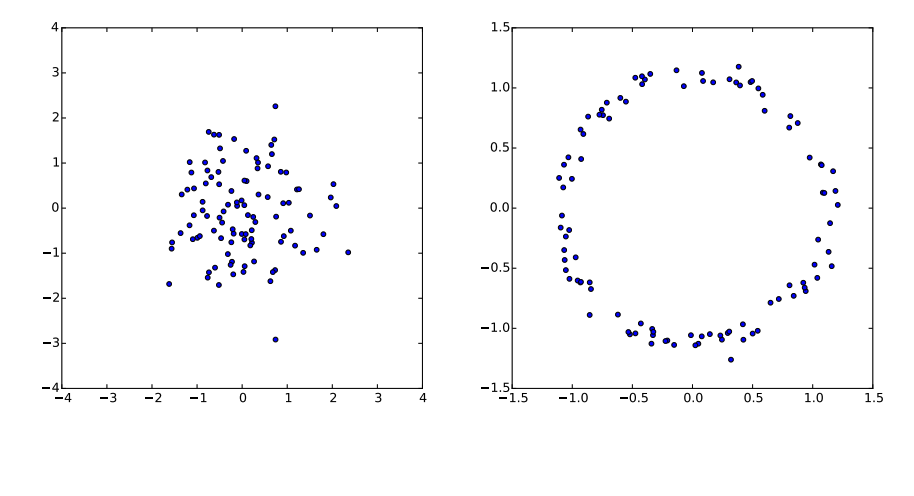
\includegraphics[width=\textwidth]{img/latent_variable_ring_structure.png}
    \caption{Máme-li náhodnou proměnnou $z$ s nějakým rozdělením pravděpodobnosti, můžeme z ní vytvořit zcela novou náhodnou proměnnou $X = g(z)$ s kompletně jiným rozdělením.}
    Levý obrázek zachycuje vzorky z Gaussova rozdělení. Pravý obrázek zachycuje ty stejné vzorky mapované skrze funkci $g(z) = \frac{z}{10} + \frac{z}{\| z \|}$.
    Obrázek včetně interpretace převzaty z \cite{Doersch2021}.
    \label{fig:latent_variable_ring_structure}
\end{figure}

Tedy, má-li VAE k dispozici dostatečně silnou aproximační funkci, může se ze vstupních dat jednoduše naučit funkci, která mapuje nezávislé hodnoty $z$ s normálním rozdělením na libovolné latentní proměnné, které jsou pro model potřebné.
VAE pak takové latentní proměnné mapuje na $X$.   \cite{Doersch2021}

Připomeňme, že (z \autoref{sec:maximum_likelihood}) $P(X|z;\theta) = \mathcal{N}(X|f(z;\theta), \sigma^2 * I)$.
Pokud je $f(z;\theta)$ Vícevrstvý Perceptron (viz \autoref{sec:multilayer_perceptron}), pak si lze intuitivně představit, že jeho umělá neuronová síť využívá svých prvních pár vrstev k mapování normálně rozdělených $z$ na latentní hodnoty (jako např. identita číslice, tloušťka tahu, sklon číslice apod.).
Pozdější vrstvy této sítě mohou být využity k mapování těchto latentních proměnných na obrázek ručně psané číslice (a to sice zcela nově vygenerovaných z pravděpodobnostního rozdělení, viz \autoref{sec:vae_generating_new_data}).
Důležité je, že (obecně) nemusíme řešit zda-li taková latentní struktura ve vstupních datech vůbec existuje.
Pokud nějaká latentní struktura pomáhá modelu s vysokou mírou přesnosti rekonstruovat (tedy optimalizovat ztrátovou funkci, viz \autoref{sec:vae_optimization}) data z trénovací množiny, pak se umělá neuronová síť tuto strukture v \emph{nějaké}\footnote{Za předpokladu dostatečně vysoko-kapacitní umělé neuronové sítě.} vrstvě naučí. \cite{Doersch2021}



\section{Enkodér modul}
\label{sec:vae_encoder}
V \autoref{sec:latent_variable_models} byly představeny hluboké modely využívající latentních proměnných (DLVM).
U těchto modelů je problém provést odhad log-likelihood a rozdělení posteriorní pravděpodobnosti. \cite{Kingma2019}

Rámec VAE poskytuje výpočetně efektivní způsob, kterým lze DLVM společně optimalizovat s jejich korespondujícími inferenčními modely pomocí stochastického gradientního sestupu
\footnote{Společně optimalziovat (\emph{joint optimization}) zde znamená, že generativní model (který mapuje latentní proměnná na data) a inferenční model (který mapuje data na latentní proměnné) jsou optimalizovány zároveň (raději než optimalizovány nezávisle). Ztrátová funkce, která je při trénování optimalizována, zahrnuje oba modely. Touto společnou optimalizací se VAE mohou učit generovat nové vzorky dat, které mají podobné vlastnosti jako data v trénovací množině a odvozovat skryté latentní vztahy proměnných, která generovala pozorovaná data}. \cite{Kingma2019}

Enkodér modul VAE je pravděpodobnostní enkodér $q_\phi(\textbf{z}\mid\textbf{x})$, který na základě datového bodu $\textbf{x}$ produkuje rozdělení pravděpodobnosti (typicky Gaussovo) skrze všechny možné hodnoty kódu $\mathbf{z}$, z něhož tento datový bod teoreticky mohl být vygenerován.  \cite{Kingma2019}

Posteriorní inference a úlohy učení DLVM jsou efektivně neřešitelné problémy.
VAE \textbf{představuje parametrický inferenční model} (\emph{parametric inference model}) $q_\phi(\textbf{z}\mid\textbf{x})$ pro přetavení těchto problémů na efektivně řešitelné.
Tento model také nazýváme \textbf{enkodér} či \textbf{rozpoznávací model}.
$\phi$ označuje parametry tohoto inferenčního modelu, tyto parametry nazýváme \textbf{variační parametry}. \cite{Kingma2019}


Variační parametry $\phi$ optimalizujeme tak, aby platila aproximace \cite{Kingma2014}:
\begin{equation}
    q_\phi(\textbf{z}\mid\textbf{x}) \approx p_\theta(\textbf{z}\mid\textbf{x})
\end{equation}

Tato aproximace posteriorního rozdělení pomáhá k optimalizaci \emph{marginal likelihood}.

Stejně jako u DLVM, inferenční model (enkodér) může být (téměř) libovolný orientovaný pravděpodobnostní grafický model \cite{Kingma2019}:
\begin{equation}
    q_\phi(\textbf{z}\mid\textbf{x}) = q_\phi(\textbf{z}_1,\dots,\textbf{z}_M\mid\textbf{x}) = \prod_{j=1}^{M} q_\phi(\textbf{z}_j\mid Pa(\textbf{z}_j), \textbf{x})
\end{equation}

kde $Pa(\textbf{z}_j)$ je množina rodičovských proměnných k proměnné $\textbf{z}_j$ v orientovaném grafu.
Podobně jako u DLVM, rozdělení pravděpodobnosti $q_\phi(\textbf{z}\mid\textbf{x})$ může být parametrizováno použitím umělé neuronové sítě (viz \autoref{fig:vae_nn}).
V takovém případě variační parametry $\phi$ zahrnují váhy a biasy této umělé neuronové sítě \cite{Kingma2014}:


\begin{align}
    (\boldsymbol{\mu}, \log \boldsymbol{\sigma}) &= \text{EnkodérSíť}_\phi(\textbf{x}) \\
    q_\phi(\textbf{z}\mid\textbf{x}) &= \mathcal{N}(\textbf{z}; \boldsymbol{\mu}, \text{diag}(\boldsymbol{\sigma})) \label{eq:enkoder_diag}
\end{align}

Pro posteriorní inferenci skrze všechna vstupní data je použita vždy jedna stejná enkodér neuronová síť, tedy \textbf{variační parametry jsou sdíleny}
\footnote{V kontrastu s tradičními metodami pro variační inferenci, kde jsou parametry iterativně optimalizovány pro každý datový vstup}.
Tato strategie, kterou VAE využívá pro \textbf{sdílení variačních parametrů skrze všechny datové vstupy} se nazývá \textbf{amortizovaná variační inference} \cite{Gershman2014}.
Amortizovanou inferencí se VAE vyhýbají optimalizační smyčce pro každý datový bod, a mohou tak plně využít možnosti efektivity stochastického gradientního sestupu. \cite{Kingma2019}
\section{Dekodér modul}
\label{sec:vae_decoder}
Dekodér modul VAE je pravděpodobnostní dekodér $p_\theta(\textbf{x}\mid\textbf{z})$,
který na základě \emph{kódu} \textbf{z} produkuje rozdělení pravděpodobnosti skrze všechny možné hodnoty, kterých může $\textbf{x}$ nabývat.
Aproximace posteriorního rozdělení generativního modelu původních dat $p_\theta(x, z)$. \cite{Kingma2014}
\newpage
\section{Evidence Lower Bound}
\label{sec:vae_objective}
Účelovou funkcí VAE je \emph{evidence lower bound}, dále jen ELBO (alternativně se lze setkat s pojmenováním \emph{variační dolní mez}).
Typicky je ELBO odvozena pomocí Jensenovy nerovnosti \cite[Sekce 4.2]{Wasserman2013}.
Autoři VAE \cite{Kingma2014} však využívají alternativního postup, jenž se chytře vyhýbá použití Jensenovy nerovnosti a nabízí větší míru \emph{tightness}
\footnote{Koncept z matematické teorie míry, který lze intuitivně popsat jako \emph{"prostor je označen za tight, pokud se prostor neroztahuje neúměrně rychle k rostoucí velikosti vzorku"}. \cite{Topsoee1974}}. 

\subsection{Odvození rovnice ELBO}
Postup odvození rovnice ELBO je převzat z monografie \textcite{Kingma2019}, rovnice jsou postupně upraveny za účelem izolování hodnoty ELBO a KL divergence, pro možnost jejich \emph{balancování} při trénovací fázi modelu.

\begin{align}
    \log p_\theta(\textbf{x}) &= \mathds{E}_{q\phi(\textbf{z}\mid\textbf{x})}[\log p_\theta(\textbf{x})] \\
                              &= \mathds{E}_{q\phi(\textbf{z}\mid\textbf{x})} \left[ \log \left[ \frac{p_\theta(\textbf{x}, \textbf{z})}{p_\theta(\textbf{z}\mid\textbf{x})} \right] \right] \\
                              &= \mathds{E}_{q\phi(\textbf{z}\mid\textbf{x})} \left[ \log \left[ \frac{p_\theta(\textbf{x}, \textbf{z})}{q_\phi(\textbf{z}\mid\textbf{x})} \frac{q_\phi(\textbf{z}\mid\textbf{x})}{p_\theta(\textbf{z}\mid\textbf{x})} \right] \right] \\
                              &= \underbrace{ \mathds{E}_{q\phi(\textbf{z}\mid\textbf{x})} \left[ \log \left[ \frac{p_\theta(\textbf{x}, \textbf{z})}{q_\phi(\textbf{z}\mid\textbf{x})} \right] \right] }_\text{$ \iff \mathcal{L}_{\theta,\phi}(\textbf{x}) (ELBO)$} 
                              +  \underbrace{ \mathds{E}_{q\phi(\textbf{z}\mid\textbf{x})} \left[ \log \left[ \frac{q_\phi(\textbf{z}\mid\textbf{x})}{p_\theta(\textbf{z}\mid\textbf{x})} \right] \right] }_\text{$\iff D_{KL}(q_\phi(\textbf{z}\mid\textbf{x})\parallel p_\theta(\textbf{z}\mid\textbf{x}))$} \\ \label{eq:elbo_kl}
\end{align}

Druhý prvek \autoref{eq:elbo_kl} je Kullback-Lieblerova divergence (\autoref{sec:kl_divergence}) mezi $q_\phi(\textbf{z}\mid\textbf{x})$ (enkodérem) a $p_\theta(\textbf{z}\mid\textbf{x})$ (dekodérem), jejíž hodnota je \textbf{nezáporná}
\footnote{$\mathcal{D}_{KL}(q_\phi(\textbf{z}\mid\textbf{x})\parallel p_\theta(\textbf{z}\mid\textbf{x})) \geq 0$}.
Je-li hodnota této KL divergence nulová, pouze pak platí, že $q_\phi(\textbf{z}\mid\textbf{x})$ je rovno posteriorní distribuci původních dat (\emph{perfektně je rekonstruuje}). \cite{Kingma2019}


První prvek \autoref{eq:elbo_kl} je variační dolní mez (ELBO), kterou lze přepsat jako:

\begin{equation} \label{eq:elbo}
    \mathcal{L}_{\theta,\phi}(\textbf{x}) = \mathds{E}_{q\phi(\textbf{z}\mid\textbf{x})}[\log p_\theta(\textbf{x},\textbf{z}) - \log q_\phi(\textbf{z}\mid\textbf{x})]
\end{equation}

S ohledem na nenulovost KL divergence je tedy ELBO \textbf{dolní mezí}\footnote{Od tud \emph{evidence \textbf{lower bound}}} log-likelihood původních dat. \cite{Kingma2014}, \cite{Goodfellow2016}
Dle \autoref{eq:elbo} platí:

\begin{align}
    \mathcal{L}_{\theta,\phi}(\textbf{x}) &= \log p_\theta(\textbf{x}) - D_{KL}(q_\phi(\textbf{z}\mid\textbf{x})\parallel p_\theta(\textbf{z}\mid\textbf{x})) \\ \label{eq:vae_optimization_objective}
                                          &\leq \log p_\theta(\textbf{x})
\end{align}

Pro libovolnou konfiguraci inferenčního modelu $q_\phi(\textbf{z}\mid\textbf{x})$, včetně volby variačních parametrů $\phi$, dostáváme \cite[Rovnice 3]{Kingma2014}:

\begin{equation}
    \label{eq:vae_elbo}
    \mathcal{L}(\theta,\phi,x^{(i)}) = \mathds{E}_{q_\phi(z\mid x^{(i)})} \left[ \log p_\theta(x^{(i)}\mid z) \right] - \mathcal{D}_{KL}(q_\phi(z\mid x^{(i)})\parallel p_\theta(z))
\end{equation}

\autoref{eq:vae_elbo} je pro \textbf{variační autoenkodéry naprosto stěžejní} a slouží jako jádro pro jejich optimalizaci
\footnote{Historicky, matematický aparát \autoref{eq:vae_elbo} byl známý dlouho před formalizací VAE. Například Helmholtz Machines \cite{Dayan1995} využívají defacto identickou rovnici, ale s jedním zásadním rozdílem. Integrál v středních hodnotách VAE je v \cite[Rovnice 5]{Dayan1995} nahrazen sumou, jelikož Helmholtz Machines usuzují diskrétní rozdělení pravděpodobnosti pro latentní proměnné. A přesně tato volba znemožňuje transformaci, kterou VAE využívají k tomu, aby byl gradientní sestup ELBO efektivně řešitelný (tractable). \cite{Doersch2021}}. \cite{Doersch2021}

V tomto případě pozoruhodně KL divergence určuje hned dvě \emph{vzdálenosti} \cite{Kingma2019}:
\begin{enumerate}
    \item KL divergenci aproximace posteriorního rozdělení od původního posteriorního rozdělení (z definice KL divergence)
    \item \emph{Mezeru} mezi ELBO $\mathcal{L}_{\theta,\phi}(\textbf{x})$ a \emph{marginal likelihood} $\log p_\theta(\textbf{x})$. Tuto \emph{mezeru} také nazýváme mírou \emph{tightness} této meze ($\implies$ vyhnutí se použití Jensenově nerovnosti). Čím lépe $q_\phi(\textbf{z}\mid\textbf{x})$ aproximuje $p_\theta(\textbf{z}\mid\textbf{x})$, s ohledem na KL divergenci, tím menší tato \emph{mezera} je.
\end{enumerate}

Schématické zobrazení \autoref{eq:vae_elbo} nabízí \autoref{fig:vae_schema}.

\begin{figure}[H]
    \centering
    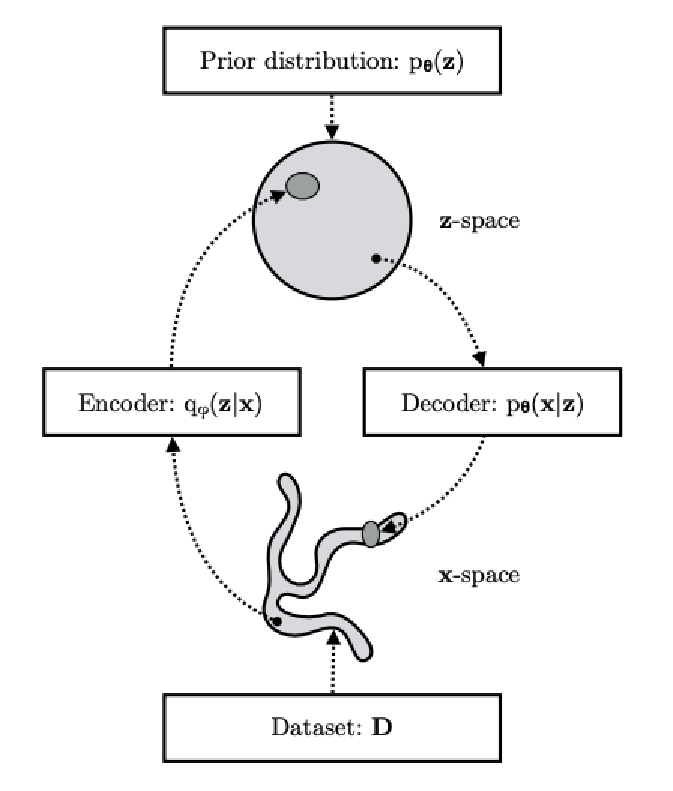
\includegraphics[width=0.41\textwidth]{figures/vae_schema.pdf}
    \caption{VAE se učí stochastické mapování mezi pozorovaným prostorem $x$, jehož empirické rozdělení pravděpodobnosti $q_\mathcal{D}(x)$ je typicky velmi komplikované, a latentním prostorem $z$, jehož rozdělení pravděpodobnosti je typicky relativně jednoduché (např. kulovité, jako na tomto obrázku). Generativní model se učí rozdělení pravděpodobnosti $p_\theta(x, z)$ (které lze faktorizovat jako $p_\theta(x, z) = p_\theta(z) p_\theta(x\mid z)$), s apriorním rozdělením skrze latentní prostor $p_\theta(z)$, a stochastický dekodér $p_\theta(x\mid z)$. Stochastický enkodér $q_\phi(z\mid x)$ aproximuje původní (ale efektivně neřešitelné) posteriorní rozdělení $p_\theta(z\mid x)$ generativního modelu. Obrázek včetně interpretace převzat z \cite{Kingma2019}.}
    \label{fig:vae_schema}
\end{figure}



\subsection{Optimalizační cíle}
Z \autoref{eq:vae_elbo} plynou důsledky maximalizace ELBO $\mathcal{L_{\theta,\phi}}$ s ohledem na parametry $\boldsymbol{\theta}$ a $\boldsymbol{\phi}$.
A to sice současná optimalizace dvou kritérií, která jsou pro výkonnost VAE stěžejní \cite{Kingma2019}:

\begin{enumerate}
    \item \emph{Přibližná} maximalizace marginální věrohodnosti $p_\theta(\textbf{x})$, což implikuje \emph{zlepšení} generativního modelu \footnote{Tedy \emph{věrohodnosti} rekonstrukce původních dat}.
    \item Minimalizace KL divergence aproximace mezi $q_\phi(\textbf{z}\mid\textbf{x})$ a původní posteriorní distribucí $p_\theta(\textbf{z}\mid\textbf{x})$. Tedy $q_\phi(\textbf{z}\mid\textbf{x})$ (enkodér) se \emph{zlepší}.
\end{enumerate}
\section{Optimalizace pomocí stochastického gradientního sestupu}
\label{sec:vae_optimization}

Za účelem optimalizace pravé strany \autoref{eq:vae_elbo} je nutné specifikovat tvar, kterého bude $q_\phi(z\mid x)$ nabývat.

Zvolíme $q_\phi(z\mid x) = \mathcal{N}(z\mid \mu(X;\theta),\Sigma(X;\theta))$, kde $\mu$ a $\Sigma$ jsou libovolné \textbf{deterministické} funkce s parametry $\theta$, které se lze učit z dat.
Funkce $\mu$ a $\Sigma$ jsou (typicky) implementovány umělou neuronovou sítí, s tím že $\Sigma$ musí být reprezentována diagonální maticí (viz \autoref{eq:enkoder_diag}).
Takto zvolené $Q(z\mid X)$ má zejména \textbf{výpočetní výhodu} – pravá strana rovnice je nyní jednoznačně spočitatelná.

Nyní je tedy poslední prvek pravé strany, $\mathcal{D}_{KL}\left[ Q(z \mid X)\parallel P(z\mid X) \right]$, KL divergence mezi dvěma vícerozměrnými Gaussovými rozděleními.
Takovou KL divergenci lze spočítat v uzavřeném tvaru následovně:

\begin{equation}\label{eq:vae_objective_long_form}
    \mathcal{D}_{KL} \left[ \mathcal{N}(\mu(X), \Sigma(X)\parallel \mathcal{N}(0, I)) \right] = 
    \frac{1}{2}\left[ \tr (\Sigma_1^{-1}\Sigma_0) + (\mu_1 - \mu_0)^\top \Sigma_1^{-1}(\mu_1 - \mu_0) - k + \log \left(\frac{\det \Sigma_1}{\det \Sigma_0} \right) \right]
\end{equation}

kde $k$ je dimenzionlita výsledného rozdělení pravděpodobnosti. \autoref{eq:vae_objective_long_form} lze dále zjednodušit následovně:

\begin{equation}
    \mathcal{D}_{KL} \left[ \mathcal{N}(\mu(X), \Sigma(X)) \parallel \mathcal{N}(0, I) \right] = 
    \frac{1}{2} \left[ \tr (\Sigma(X)) + (\mu(X))^\top (\mu(X)) - k - \log \det (\Sigma(X)) \right].
\end{equation}

První prvek pravé strany \autoref{eq:vae_elbo} je o něco komplikovanější.

Bylo by možné pomocí vzorků odhadnout $\mathds{E}_{q_\phi(z\mid x^{(i)})} \left[ \log p_\theta(x^{(i)}\mid z) \right]$, ale pro získání \emph{věrohodného} odhadu je nutné skrze $z$ poslat velké množství vzorků, což je výpočetně náročné.
Tedy, jak je u stochastického gradientního sestupu běžné, využijeme pouze jeden vzorek $z$ a použijeme $P(X\mid z)$ pro toto $z$ jako aproximaci této střední hodnoty
\footnote{Zde je výhodou, že provést stochastický gradientní sestup skrze všechny různé hodnoty $X$ vzorkované z datové sady $D$ již stochastický gradientní sestup provádíme při trénování.}.


Tedy \textbf{rovnice kterou chceme optimalizovat} má následující podobu:

\begin{align}
   \nabla_\phi \mathcal{L}_{\theta,\phi}(x) &= \nabla_\phi \mathds{E}_{q_\phi(z\mid x)} \left[ \log p_\theta (x, z) - \log q_\phi (z\mid x) \right] \label{eq:vae_final_objective} \\
                                            &\neq \mathds{E}_{q_\phi(z\mid x)} \left[ \nabla_\phi (\log p_\theta (x, z) - \log q_\phi (z\mid x) ) \right] \label{eq:vae_final_objective_dependent_gradient}
\end{align}

Symbol gradientu této může být bezpečně přesunut do střední hodnoty.
Tedy, můžeme vzorkovat jednu hodnotu z $X$ a jednu hodnotu ze $z$ z a následně vypočítat gradient:

\begin{equation} \label{eq:sample_gradient}
    \log p_\theta(x \mid z) - D_{KL}(q_\phi(\textbf{z}\mid\textbf{x})\parallel p_\theta(\textbf{z})). 
\end{equation}

Průměr gradientu této funkce skrze \emph{libovolně velké} množství vzorků z $x$ a $z$. Výsledná hodnota tohoto gradientu konverguje ke gradientu \autoref{eq:vae_final_objective}.

\subsection{Metoda stochastická gradientní optimalizace ELBO}
Důležitou vlastností ELBO je možnost \emph{joint} optimalizace s ohledem na veškeré její parametry – $\boldsymbol{\phi}$ a $\boldsymbol{\theta}$ – za použití stochastického gradientního sestupu (\emph{stochastic gradient descent, SGD}).
Proces lze zahájit náhodnými počátečními hodnotami $\boldsymbol{\phi}$ a $\boldsymbol{\theta}$ a stochasticky optimalizovat jejich hodnoty než dojde ke konvergenci.

Mějme nezávisle a rovnoměrně rozdělená vstupní data, účelovou funkcí ELBO je součet ELBO jednotlivých datových bodů:
\begin{equation}
    \mathcal{L}_{\theta,\phi}(\mathcal{D}) = \sum_{x\in\mathcal{D}}^{} \mathcal{L}_{\theta,\phi}(\textbf{x})
\end{equation}

ELBO jednotlivých datových bodů a jejich gradienty jsou \emph{obecně} efektivně řešitelné.
Dokonce existují estimátory bez biasu, za pomocí kterých lze provést minibatch SGD.

Gradienty ELBO bez biasu s ohledem na parametry generativního modelu $\boldsymbol{\theta}$ lze jednoduše získat (viz rovnice 2.14 - 2.17 z \cite{Kingma2019}).

Spočítat gradienty ELBO bez biasu s ohledem na variační parametry $\boldsymbol{\phi}$ je již složitější, jelikož tato ELBO je uvažována s ohledem na rozdělení pravděpodobnosti $q_\phi(\textbf{z}\mid\textbf{x})$, tedy je funkcí $\phi$. Nerovnost gradientů ELBO viz rovnice 2.18 - 2.19 z \cite{Kingma2019}.

V případě \textbf{spojitých} latentních proměnných lze využít tzv. \textbf{reparametrizačního triku} pro výpočet odhadů bez biasu $\nabla_{\theta,\phi}\mathcal{L}_{\theta,\phi}(\textbf{x})$.
Tento stochastický odhad umožňuje optimalizovat ELBO za SGD (viz \autoref{alg:reparam_trick})
\footnote{Existují i metody pro případ \textbf{diskrétních} latentních proměnných, které však pro předmět práce nejsou stěžejní. Pro jejich představení odkazuji na \cite[Sekce 2.9.1.]{Kingma2019}.}.

\begin{algorithm}[H]
    \caption{Stochastická optimalizace variační dolní meze (ELBO).}\label{alg:reparam_trick}
        \KwData{}
                \hspace{6mm}$\mathcal{D}$: Dataset (i. i. d.)\\
                \hspace{6mm}$q_\phi(\textbf{z}\mid\textbf{x})$: Inferenční model (enkodér)\\
                \hspace{6mm}$p_\theta(\textbf{x}, \textbf{z})$: Generativní model (dekodér)\\
        \KwResult{}
        \hspace{6mm}$\boldsymbol{\theta}, \boldsymbol{\phi}$: Naučené parametry\\

        $\boldsymbol{\theta}, \boldsymbol{\phi} \gets \text{Náhodná inicializace parametrů}$

        \While{SGD not converged}{
            $\mathcal{M} \sim \mathcal{D}$ (Random minibatch of data)\\
            $\boldsymbol{\epsilon} \sim p(\boldsymbol{\epsilon})$ (Random noise for every datapoint in $\mathcal{M}$)\\
            Compute $\tilde{\mathcal{L}}$ and its gradients $\nabla_{\theta,\phi}(\mathcal{M}, \boldsymbol{\epsilon})$\\
            Update $\boldsymbol{\theta}$ and $\boldsymbol{\phi}$ using SGD optimizer
            }
\end{algorithm}

Aby VAE fungovaly dle očekávání, $q_\phi(z\mid x)$ musí být nuceno produkovat takové kódy pro $x$, které bude $p_\theta(x, z)$ schopno \textbf{spolehlivě} dekódovat.
Na tento problém lze alternativně pohlížet interpretací \autoref{eq:vae_final_objective} jako sítě vyobrazené TODO FIGURE NO-BACKPROP.
Dopředný průchod této sítě funguje bez problémů – a je-li její výstup zprůměrován skrze mnoho vzorků $x$ a $z$, produkuje správnou střední hodnotu.
Nicméně, je nutné mít schopnost zpětně propagovat chybu skrze vrstvu, která vzorkuje $z$ z $q_\phi(z \mid Xx$, což je \textbf{nespojitá operace} a tedy nemá žádný gradient.
Stochastický gradientní sestup se zpětnou propagací zvládne stochastické vstupy, ale \textbf{neumí pracovat se stochastickými jednotkami (neurony) sítě}.

Řešení tohoto problému nazýváme \textbf{reparametrizační trik}.
\section{Reparametrizační trik}
\label{sec:reparametrization_trick}
Reparametrizační trik spočívá v přesunutí procesu vzorkování do vstupní vrstvy. \cite{Doersch2021}

Reparametrizační trik \emph{funguje} pouze pakliže lze vzorkovat z $Q(z\mid X)$ vyhodnocením funkce $h(\eta, X)$, kde $\eta$ je šum (z distribuce jejíž parametry nejsou učeny z dat). $h$ také musí být spojitá na $X$, abychom skrze něj mohli provádět zpětnou propagaci.
To, mimo jiné, znamená, že $Q(z\mid X)$ a tím padem i $P(z)$ \textbf{nemohou být diskrétní rozdělení}. V opačném případě by došlo k nespojitosti prostoru vzorků $Q$ – a tedy neschopnosti generativního modelu generovat vzorky v celém rozsahu, včetně vzorků které nebyl součástí dat (běžný problém autoenkodérů, které uvedla \autoref{chap:autoencoder}.)

Mějme $\mu(X)$ a $\Sigma(X)$. Pak je možné vzorkovat z $\mathcal{N}(\mu(X), \Sigma(X))$ – nejprve provedeme vzorkování z $\epsilon \sim \mathcal{N}(0, I)$ a následně spočteme $z = \mu(X) + \Sigma^{\frac{1}{2}}(X) * \epsilon$. \cite{Doersch2021}
Interpretaci hodnot $\mu$ a $\sigma$ nabízí enkodér a dekodér moduly modulu variačního autoenkodéru dle \autoref{sec:vae_model_architecture}.

Finální rovnice, jejíž gradient chceme spočítat má následující tvar:

\begin{equation} \label{eq:vae_reparam_trick}
    \mathds{E}_{X \sim D} \left[ \mathds{E}_{\mathcal{N}(\epsilon; 0, 1)} \left[ \log P(X\mid z = \mu(X) + \Sigma^{\frac{1}{2}} (X) * \epsilon) \right] -  D_{KL}(q_\phi(\textbf{z}\mid\textbf{x})\parallel p_\theta(\textbf{z})) \right].
\end{equation}

\begin{figure}[H]
    \centering
    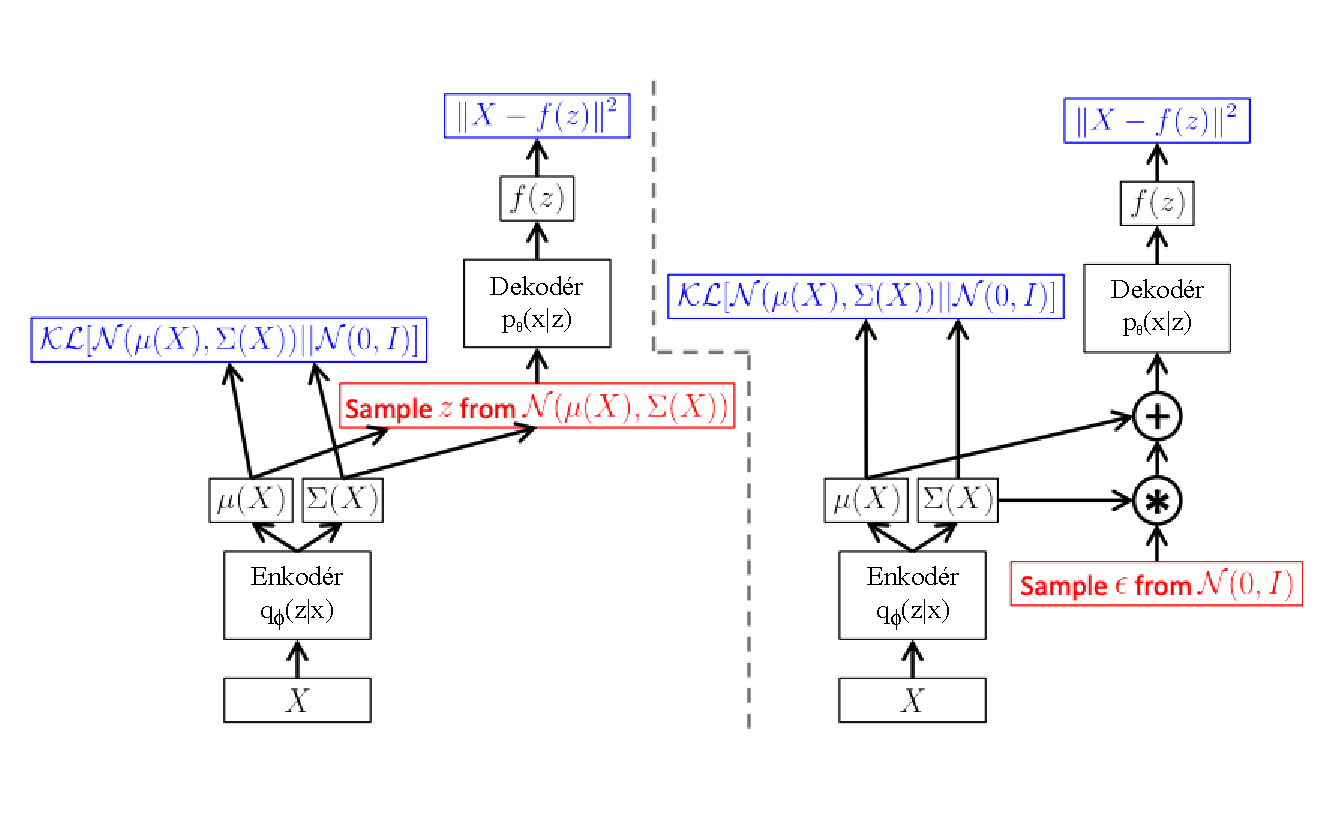
\includegraphics[width=0.8\textwidth]{figures/vae_backpropagation.pdf}
    \caption{Trénovací fáze dopředné umělé neuronové sítě VAE. Levý obrázek je znázorněn bez reparametrizačního triku. Pravý obrázek zahrnuje reparametrizační trik. Červené bloky zobrazují vzorkovací operace, které jsou nediferenciovatelné. Modré bloky zobrazují ztrátové vrstvy neuronové sítě. Dopředné chování obou sítí je \textbf{identické}, ale pouze v síti na pravém obrázku lze provést zpětná propagace. Obrázek včetně interpretace převzat z \cite{Doersch2021}.}
    \label{fig:vae_backpropagation}
\end{figure}

Kýžená vlastnost \autoref{eq:vae_reparam_trick} je, že v modelu její \textbf{umělé neuronové sítě lze provést zpětnou propagaci}
\footnote{Žádné střední hodnoty ($\mathds{E}$) \autoref{eq:vae_reparam_trick} \textbf{nezávisí} na parametrech modelu. Tedy do těchto středních hodnot můžeme bezpečně převést symbol gradientu a zároveň dodržet jejich rovnost. 
Tedy, mějme neměnné $X$ a $\epsilon$, pak je tato funkce \textbf{spojitá a deterministická} v parametrech $P$ a $Q$, což v důsledku znamená možnost zpětné propagace vypočíst gradient algoritmem stochastického gradientního sestupu.}. 
A díky tomu lze srkze model variačního autoenkodéru zpětně propagovat chyba ztrátové funkce a tím způsobem jej optimalizovat (viz \autoref{sec:multilayer_perceptron}). Toto znázorňuje \autoref{fig:vae_backpropagation}(b). \cite{Kingma2014}

\section{Tří různé pohledy na interpretaci naučeného modelu}
Jak bylo ukázáno, proces učení variačních autoenkodérů je efektivně řešitelný problém (\emph{tractable}).

Při učení je optimalizován $\log P(X)$ skrze celou množinu vstupních dat $D$. Nicméně, není optimalizován \emph{přesně} $\log P(X)$, ale pouze jeho odhad.

Tato sekce slouží pro odkrytí mechanismů, které se skutečně na pozadí účelové funkce variačního autoenkodéru dějí.
Nabízí tři různé pohledy, kterými může být \autoref{eq:vae_elbo} interpretována:
\begin{enumerate}
    \item Velikost chyby, kterou způsobuje současná optimalizace $\mathcal{D}_{KL}(q_\phi(z\mid x^{(i)})\parallel p_\theta(z))$ dodatečně vedle optimalizace $\log p_\theta(x^{(i)})$.
    \item Interpretace v kontextu informační teorie a propojení s dalšími přístupy založenými na Minimal Description Length.
    \item VAE a regularizační prvek. Existuje u variačních autoenkodérů regularizační prvek, obdobně jako u  autoenkodérů které uvedla \autoref{chap:autoencoder}?
\end{enumerate}

\subsection{Chyba $\mathcal{D}_{KL}(q_\phi(z\mid x^{(i)})\parallel p_\theta(z))$}
\textbf{Efektivní řešitelnost} modelu variačního autoenkodéru závisí na předpokladu,
že $Q(z\mid X)$ \textbf{lze modelovat jako Gaussovu funkci se střední hodnotou $\mu(X)$ a rozptylem $\Sigma(X)$}.

Rozdělení $P(X)$ konverguje k původnímu rozdělení (které generuje vstupní data) pouze když se $\mathcal{D}_{KL}(q_\phi(z\mid x^{(i)})\parallel p_\theta(z))$ limitně blíží k nule.
Což ale nelze jednoduše zaručit. Ani za předpokladu, že $\mu(X)$ a $\Sigma(X)$ jsou vysoko-kapacitní umělé neuronové sítě
\footnote{Vysoko-kapacitní neuronové sítě, jsou sítě s vysokým počtem parametrů a vah, které jim umožňují učit se komplexním vztahům mezi daty. \cite[Kapitola 5]{Goodfellow2016}}
neplatí, že posteriorní rozdělení $P(z\mid X)$ musí být vždy Gaussovo (pro libovolnou funkci $f$ která je použita pro definování $P$).
Tedy, pro neměnné $P$ to znamená, že $\mathcal{D}_{KL}(q_\phi(z\mid x^{(i)})\parallel p_\theta(z))$ \textbf{nikdy neni rovno nule} (pokud by tato KL divergence byla rovna nule, viz \autoref{eq:elbo_kl}, znamenalo by to perfektní rekonstrukci původních dat).

Nicméně, máme-li dostatečně vysoko-kapacitní neuronové sítě, existuje mnoho funkcí $f$ (viz \autoref{sec:universal_approximation_theorem}), které zaručí, že naučený model generuje libovolné výstupní rozdělení pravděpodobnosti
\footnote{Tedy je schopen generovat vzorky \emph{dostatečně podobné} vzorkům množiny trénovacích dat, včetně vzorků, které nebyly při trénování k dispozici.}.
Libovolná z těchto funkcí maximalizuje $\log P(X)$ stejně dobře. Tedy stačí vybrat jednu z těchto funkcí, která maximalizuje $\log P(X)$ \textbf{a zároveň} zaručí, že $P (z\mid X)$ je Gaussovou funkcí pro všechna $x^{(i)}$.
Pokud toto platí, $\mathcal{D}_{KL}(q_\phi(z\mid x^{(i)})\parallel p_\theta(z))$, \emph{tlačí} model směrem k parametrizaci původní distribuce.

Zbývá zodpovědět, zda-li taková funkce existuje pro všechny libovolné distribuce, které bychom mohli chtít aproximovat.
Tento problém (v kontextu variačních autoenkodérů) zatím zůstává nezodpovězen. Nicméně existuje alespoň formální důkaz \textbf{nulové chyby aproximace} VAE alespoň v triviálním teoretickém scénáři na 1D problému \cite[Příloha A]{Doersch2021}.
Autoři rámce VAE se domnívají, že budoucí teoretický výzkum by měl být schopný na tomto důkazu stavět a rozšířit jej na více (složitějších) scénářů s praktickým využitím. 

\subsection{Interpretace z pohledu informační teorie}
\label{sec:vae_information_theory_interpretation}
Dalším možným (a velmi důležitým) pohledem na pravou stranu \autoref{eq:vae_elbo} je v kontextu informační teorie.
Konkrétně pomocí principu tzv. \emph{minimum description length}, který stojí za mnoha předchůdci variačního autoenkodéru, jako například Helmholtz Machines, Wake-Sleep Algoritmus, Deep Belief Nets a Boltzmann Machines.

Na $- \log P(X)$ lze pohlížet jako na celkový počet bitů, které naučený model potřebuje k sestavení daného $x^{(i)}$ za použití \textbf{ideálního} kódování.
Pravá strana \autoref{eq:vae_elbo} na toto pohlíží jako na dvoufázový proces pro sestavení $x^{(i)}$.

V první fázi použijeme \emph{nějaký počet} bitů pro sestavení $z$ \footnote{Pro připomenut KL divergenci lze uvádět v jednotkách bitů (viz \autoref{sec:kl_divergence}).}.
Konkrétně $\mathcal{D}_{KL}(q_\phi(z\mid x^{(i)})\parallel p_\theta(z))$ je očekávaná informace potřebná pro převedení vzorku z $P(z)$ (bez informace) na vzorek z $Q(z\mid X)$ (tzv. interpretace KL divergence jako informačního zisku).
Tedy měří množství nadbytečné informace které obdržíme o $x^{(i)}$ když obdržíme $z$ ze $Q(z\mid X)$ namísto z $P(z)$
\footnote{Pro detailněji popsanou interpretaci odkazuji na "bits back" argument z TODO CITACE }.

V druhé fázi $P(X\mid z)$ měří množství informace potřebné pro rekonstrukci $x^{(i)}$ ze $z$ za použití ideálního kódování.

Tedy celkový počet bitů ($- \log P(X)$) je součtem těchto dvou fází mínus trestu, který platíme za to, že $Q$ suboptimální kódováním $\mathcal{D}_{KL}(q_\phi(z\mid x^{(i)})\parallel p_\theta(z))$. 


\subsection{VAE a regularizační prvek}
\label{sec:vae_regulariazion_term}
\autoref{eq:vae_elbo} nabízí další pohled na $\mathcal{D}_{KL}(q_\phi(z\mid x^{(i)})\parallel p_\theta(z))$ jakožto na jakýsi regularizační prvek.
Stejně jako u řídkého autoenkodéru (viz \autoref{sec:sparse_autoencoder}), kde regularizační prvek $\Omega$ penalizuje aktivaci neuronů.
Z tohoto pohledu je zajímavé zamyslet se, zda-li u variačních autoenkodérů vůbec existuje \emph{něco jako} regularizační prvek.

U variačního autoenkodéru \textbf{regularizační prvek} obecně vůbec \textbf{neexistuje}.
Což je výhodou – jelikož to znamená o jeden prvek, který je nutné optimalizovat, méně.

Nicméně, určité modely variačního autoenkodéru se jeví, že regularizační prvek \emph{existuje}
\footnote{Nabízí se zaměnit $z \sim \mathcal{N}(0, I)$ za $z^\prime \sim \mathcal{N}(0, \Sigma * I)$, ale ukázalo se že toto naučený model nijak nezmění a ve skutečnosti vyprodukuje identickou ztrátovou funkci a model pro vzorkování $x^{(i)}$. \cite{Doersch2021}}.
Dobrou volbou výstupního rozdělení pravděpodobnosti pro spojitá data je $P(X\mid z) \sim \mathcal{N}(f(z), \sigma^2 * I)$ pro libovolné $\sigma$ které předem dodáme.
Tím pádem dostáváme $\log P(X\mid z) = C - \frac{1}{2} \| X - f(z) \|^2 / \sigma^2$, kde $C$ je konstanta, která nezávisí na $f$ a tak ji lze při optimalizaci zanedbat.

Pokud toto rozdělení pravděpodobnosti použijeme, ve výsledné účelové funkci se $\sigma$ objeví jako druhý prvek na pravé straně \autoref{eq:vae_elbo}.
Tedy v tomto smyslu lze zvolené $\sigma$ svou rolí považovat za jakési $\Omega$ které kontroluje váhy obou prvků pravé strany.
Nutno podotknout, že samotná existence tohoto parametru je závislá na zvoleném rozdělení pravděpodobnosti $x^{(i)}$ pro dané $z$.
Tedy pokud je $x^{(i)}$ binární, a jako výstupní model je použito Alternativní rozdělení, tento \emph{regularizační} prvek zmizí 
\footnote{I přes to existují způsoby, jakým jej lze dostat zpět do rovnice, jako například replikace dimenzí $x^{(i)}$. \cite{Doersch2021}}.
Což z pohledu informační teorie dává logiku: je-li $x^{(i)}$ binární, lze spočítat počet bitů, které jsou potřebné pro kódování $x^{(i)}$, a tím pádem oba prvky pravé strany \autoref{eq:vae_elbo} používají stejné jednotky.
Nicméně, pokud je $x^{(i)}$ spojité, každý vzorek obsahuje nekonečnou míru informace. Volba $\sigma$ pak určuje očekávanou míry přesnosti, s jakou je naučený model schopen rekonstruovat $x^{(i)}$, resp. celé $X$. (tento kompromis je nutný, aby se míra informace vzorku stala konečná).

\section{Generování nových vzorků}
\label{sec:vae_generating_new_data}
Pro vygenerování nového vzorku $\textbf{\emph{x}}$ z modelu VAE je nejprve nutné získat vzorek $\textbf{\emph{z}}$ z rozdělení pravděpodobnosti kódu $p_{model}(\textbf{\emph{z}})$.
Poté je tento vzorek vstupem pro síť generátoru $g(\textbf{\emph{z}})$. Na konec je $\textbf{\emph{x}}$ vzorkováno z rozdělení pravděpodobnosti $p_{model}(\textbf{\emph{x}};g(\textbf{\emph{z}})) = p_{model}(\textbf{\emph{x}}\mid\textbf{\emph{z}})$. \cite{Kingma2014}

Při trénování je však pro získání $\textbf{\emph{z}}$ použit enkodér (\emph{approximate inference network}) $q(\textbf{\emph{z}}\mid\textbf{\emph{x}})$ a na $p_{model}(\textbf{\emph{x}}\mid\textbf{\emph{z}})$ pak lze pohlížet jako na dekodér. \cite{Kingma2014}

Klíčovým principem VAE je, že může být trénován maximalizací variační dolní meze (\emph{variational lower bound}) $\mathcal{L}(q)$ asociovanou s datovým bodem $\textbf{\emph{x}}$ následovně \cite{Goodfellow2016}: 

\begin{align}
    \mathcal{L}(q) &= \overbrace{ \mathds{E}_{q_\phi(z\mid x^{(i)})} \left[ \log p_\theta(x^{(i)}\mid z) \right] }^\text{společná log věrohodnost} + \overbrace{ \mathcal{H}(q(\textbf{z} \mid \textbf{\emph{x}})) }^\text{entropie} \label{eq:sampling_vae_1} \\
    &= \mathds{E}_{q_\phi(z\mid x^{(i)})} \left[ \log p_\theta(x^{(i)}\mid z) \right] + D_{KL}(q(\textbf{z} \mid \textbf{\emph{x}})\parallel p_{model}(\textbf{z}))) \label{eq:sampling_vae_2} \\
    &\leq \log p_{model}(\textbf{\emph{x}})
\end{align}

První člen \autoref{eq:sampling_vae_1} ukazuje společnou log věrohodnost (\emph{log-likelihood)} viditelných a skrytých proměnných pod \emph{approximate posterior} skrze latentní proměnné (stejně jako u EM, s rozdílem že používáme \emph{approximate} místo \emph{exact} posterior). \cite{Goodfellow2016}

Druhý člen \autoref{eq:sampling_vae_1} ukazuje entropii \emph{approximate posterior}.
Je-li $q$ Gaussova distribuce, a je-li k predikované střední hodnotě přičten šum, maximalizace této entropie vede k zvyšující se směrodatné odchylce tohoto šumu.
Obecně, prvek této entropie zajistí tendenci \emph{variational posterior} přidělit vysokou hodnotu funkce pravdepodobnostni hodnotám $\textbf{\emph{z}}$ které by mohly generovat $\textbf{\emph{x}}$ (raději než konvergovat pouze k odhadu jedné hodnoty s \emph{největší pravděpodobností}). \cite{Goodfellow2016}

První člen \autoref{eq:sampling_vae_2} ukazuje log věrohodnost rekonstrukce, který lze nalézt i v ostatních typech autoenkodérů (\autoref{chap:autoencoder}). 

Druhý člen \autoref{eq:sampling_vae_2} zajišťuje, aby se \emph{approximate posterior distribution} $q(\textbf{z}\mid\textbf{\emph{x}})$ a model prior $p_{model}(\textbf{\emph{z}})$ k sobě blížily. \cite{Goodfellow2016}

Tradiční přístupy k variačnímu odvozování a učení odvozují $q$ pomocí optimalizačního algoritmu (typicky iterují skrze soustavy \emph{fixed-point} rovnic).
Takové přístupy jsou pomalé a výpočetně neefektivní, jelikož často vyžadují schopnost vypočítat $\mathds{E}_{\textbf{\emph{z}} \sim q}$ v uzavřeném tvaru. \cite{Goodfellow2016}

\textbf{Hlavní myšlenkou variačních autoenkodérů je natrénování parametrického autoenkodéru} (také nazývaného jako \emph{odvozovací síť} či \emph{rozpoznávací model}) \textbf{který produkuje parametry $\textbf{q}$}.
Je-li $\textbf{\emph{z}}$ spojitá proměnná, lze vždy provést algoritmus zpětné propagace skrze vzorky $\textbf{\emph{z}}$ získané z $q(\textbf{\emph{z}}\mid\textbf{\emph{x}}) = q(\textbf{\emph{z}};f(\textbf{\emph{x}}; \bm{\emph{$\theta$}}))$ za účelem spočtení gradientu s respektem k $\bm{\emph{$\theta$}}$. \cite{Goodfellow2016}

\textbf{Učení VAE pak spočívá čistě v maximalizaci $\mathcal{L}$ s ohledem na parametry enkodéru a dekodéru}. \cite{Kingma2014}
\section{Testování naučeného modelu}
Pro testování modelu chceme generovat nové vzorky – toho lze dosáhnout použitím hodnot ze $z \sim \mathcal{N}$ jako vstup pro dekodér.
Jedná se tedy vlastně o odstranění enkodéru (včetně operací násobení a sčítání, které by jinak měnily rozdělení pravděpodobnosti $z$).

Schéma této jednoduché sítě je vyobrazeno v TODO FIGURE TEST-TIME NETWORK.

Chceme-li vyhodnotit pravděpodobnost vygenerování konkrétního vzorku z naučeného modelu, jedná se o efektivně neřešitelný problém (tento problém je adresován pomocí tzv. Podmíněných variačních autoenkodérů).

\subsubsection{Lower bound}
Evidence lower bound však poskytuje alespoň hrubý odhad toho, jak naučený model zachycuje konkrétní datový bod $X$.

$\mathcal{D}_{KL}\left[ Q(z\mid X) \parallel P(z\mid X) \right]$ má nezápornou hodnotu (viz \autoref{sec:evidence_lower_bound}).
Tedy pravá strana rovnice \autoref{eq:vae_objective} je dolní mezí $P(X)$.

Ale i tato dolní mez stále nelze vypočítat v uzavřeném tvaru (z důvodu závislosti očekávané hodnoty na $z$, což opět znamená nutnost vzorkování).
Nicméně, vzorkování $z$ z $Q$ dává estimátor pro očekávanou hodnotu, což alespoň konverguje mnohem rychleji, než vzorkování z $\mathcal{N}(0, I)$ (viz \autoref{chap:vae}).

 \section{Nedostatky a omezení}
Variační autoenkodér nabízí elegantní a po teoretické stránce uspokojivý přístup, který je jednoduchý na implementaci.
V oblasti generativního modelování dosahuje excelentních výsledků, ale s ohledem na jeho architekturu přichází i několik podstatných nedostatků.
\subsection{Omezení při optimalizaci}
Nálezy v \cite{Bowman2016}, \cite{Soenderby2016} konzistentně potvrzují, že stochastická optimalizace účelové funkce s neměnnou dolní mezí může uvíznout v nežádoucí rovnováze.
Při počátku trénování je pravděpodobnostní prvek $\log p(x\mid z)$ relativně slabý, tedy je přípustný stav kdy $q(z \mid x) \approx p(z)$ – což je přesně bod, kdy tato nežádoucí rovnováha nastává a je složité z ní při optimalizaci uniknout.

Řešení navrhované v \cite{Bowman2016} a \cite{Soenderby2016} využívá rozvrhování optimalizace tak, že váhy latentního \emph{nákladového kritéria} $\mathcal{D}_{KL}(q_\phi(z\mid x^{(i)})\parallel p_\theta(z))$ jsou při trénování skrze mnoho epoch \emph{žíhány} v intervalu od 0 do 1.
Tento přístup staví na metodě simulovaného žíhání, která představuje způsob pro uniknutí z lokálního extrému při optimalizaci (gradientním sestupem). \cite{Kirkpatrick1983}

Alternativní řešení, navrhované v \cite{Kingma2016}, je tzv. metoda \emph{free bits}. Jedná se o jakousi modifikaci ELBO (viz \autoref{eq:vae_elbo}) účelové funkce,
která zaručí, že v průměru je v každé latentní proměnné (nebo skupině latentních proměnných) zakódováno \textbf{alespoň} určité minimální množství bitů informace.


\subsection{Šum v obrázcích vygenerovaných vzorků}
\label{sec:vae_bluriness}
Jednou z hlavních nevýhod variačního autoenkodéru, zejména v kontextu úloh generativního modelování obrazových dat, je fakt, že výstupní vzorky z VAE natrénovaného na obrazových datech mají tendenci být rozostřeny.
Jednou z možných příčin by mohl být důsledek minimalizace $D_{KL}(p_{data}\parallel p_{model})$ (zjednodušený zápis pro jednoduchost).
Takto natrénovaný model přidělí vysokou pravděpodobnost bodům, které jsou součástí trénovací množiny dat, ale i \emph{spoustě} dalších bodů (vzorků, které generuje z naučeného Gaussova rozdělení). A právě tyto vzorky, které nebyly součástí trénovací množiny dat, často obsahují šum a jeví se tak jako rozostřené. \cite{Goodfellow2016}

Přesné příčiny tohoto problému však zatím nejsou známy. Přirozeně tak vzniká celá řada nových, rozšířených architektur variačního autoenkodéru, která svými omezeními tento problém to jisté míry eliminují.
\section{Aktuální stav poznání a rozšíření variačního autoenkodéru}
\label{sec:vae_extensions}
Tato sekce nabízí přehled technik, které se svým principem podobají variačním autoenkoderům a prezentuje jejich odlišnosti.
\subsection{Wake-sleep algoritmus}
Wake-sleep algoritmus \cite{Hinton1995} je další on-line metodou pro učení, která je aplikovatelná na stejnou třídu modelů využívajících latentních proměnných, jako VAE.
Obdobně jako VAE (\autoref{sec:vae_encoder}), wake-sleep algoritmus využívá recognition model který aproximuje posteriorní rozdělení původních dat.
Značnou nevýhodou wake-sleep algoritmu oproti VAE však je nutnost současné optimalizace dvou účelových funkcí, které dohromady nekorespondují s optimalizací dolní meze marginální věrohodnosti.
Výhodou wake-sleep algoritmu oproti VAE je, že je také aplikovatelný na modely s diskrétními latentními proměnnými.
Wake-sleep algoritmus rovněž nabízí stejnou výpočetní složitost skrz jeden datový bod jako ELBO. \cite{Kingma2019}

\subsection{Regularizované autoenkodéry}
Rozšířením \autoref{sec:denoising_autoencoder} a \autoref{sec:stacked_autoencoder} jsou Stacked Denoising Autoenkodéry \cite{Vincent2010}. Jejich princip spočívá v maximalizaci (s ohledem na parametry) vzájemné informace  a je ekvivalentní s maximalizací podmíněné entropie. Což je dolní mezí očekávané log-věrohodnosti dat, které jsou výstupem autoenkodér modelu – tedy tzv. \emph{negative reconstruction} chyba.
Nicméně, jak bylo ukázáno \cite{Bengio2014}, toto kritérium pro rekonstrukci dat \textbf{není dostatečné} pro naučení modelu \textbf{užitečným} reprezentací vstupních dat.

Přirozeně tedy bylo přistoupeno k regularizačním technikám, které zajistí naučení užitečných reprezentací. Tyto návrhy představují \autoref{sec:sparse_autoencoder}, \autoref{sec:denoising_autoencoder}, \autoref{sec:contractive_autoencoder} a \autoref{sec:stochastic_autoencoder}.
Možnost regularizačního prvku jako součást účelové funkce variačního autoenkodéru popisuje \autoref{sec:vae_regulariazion_term}.

\subsection{Generativní stochastické sítě}
\cite{Bengio2014a} představuje generativní stochastickou síť, kde se noisy autoenkodér učí přechodovou funkci a operátory Markovova řetězce, který vzorkuje z rozdělení pravděpodobnosti vstupních dat.  Toto vzorkování je potom využito pro sestavení generativního procesu, což je ve vztahu k variačním autoenkodérům přidružená technika. \cite{Kingma2019}

\subsection{Efektivní učení reprezentací pomocí hlubokých Boltzmann machines}
V \cite{Salakhutdinov2010} byl využit recognition model (podobně jako \autoref{sec:vae_encoder}) pro efektivní učení reprezentací pomocí hlubokých Boltzmann machines. 
Tato metoda je zaměřena pouze na nenormalizované modely (např.: Boltzmann machines) nebo řídké kódovací modely. V kontrastu s variačním autoenkodér, který je schopen učit se problémům v obecné třídě orientovaných pravděpodobnostních modelů. \cite{Kingma2019}

\subsection{Hluboké autoregresivní sítě}
Obdobně jako variační autoenkodér, \cite{Gregor2014} představuje metodu pro učení se pravděpodobnostního modelu za využití autoenkodér struktury. Nicméně navrhovaná metoda je aplikovatelná pouze při uvažování binárních latentních proměnné (v kontrastu s VAE, kde toto omezení neexistuje). \cite{Kingma2019}

\subsection{Stochastic Backpropagation and Approximate Inference in Deep Generative Models}
Práce publikována souběžně a nezávisle na autorech rámce VAE (z jejichž publikací \autoref{chap:vae} převážně čerpá). Práce \cite{Rezende2014} rovněž představuje propojení autoenkodérů, orientovaných pravděpodobnostních modelů a stochastické variační inference pomocí regularizačního triku, tedy stejných principů, které popisuje \autoref{chap:vae}.
Představuje alternativní interpretaci a vhled do vnitřní architektury variačního autoenkodéru.

\subsection{Conditional variační autoenkodér}
\label{sec:cvae}
Conditional variační autoenkodér (CVAE) \cite{Sohn2015} modifikuje matematický aparát variačního autoenkodéru, který popisuje \autoref{chap:vae}, \textbf{podmíněním celého generativního procesu na vstupu}. Tedy vytváří vazbu generativního procesu na konkrétní vstup (resp. konkrétní podobu výstupu).
CVAE nabízí řešení problému, kde má input-output mapovací funkce kardinalitu 1:n
\footnote{V textech strojového učení se můžeme setkat s pojmenováním \emph{strukturovaná predikce}.},\textbf{bez nutnosti explicitní specifikace} struktury výstupního rozdělení pravděpodobnosti.
Tedy, použijeme-li opět úlohu generování ručně psané číslice: CVAE nabízí možnost pro generování variací vstupu – tedy pokud na vstupu příjde ručně psaná číslice 9, model CVAE je schopen generovat variace ručně psané číslice 9 \textbf{které nebyly součástí trénovací množiny}.

CVAE rovněž řeší problém rozostřených výstupů generativního modelu (viz \autoref{sec:vae_bluriness}). Regresor VAE minimalizuje vzdálenost k množině mnoha různých výstupů, které potenciálně mohly generovat vstup. Naopak CVAE obecně vybere specifický výstup (např. jednu konkrétní číslici, kterou obdrží na vstupu), a tu generuje – tedy výsledkem je více \emph{realistický} vzorek této konkrétní číslice.  
\cite{Doersch2021}

\subsection{Deep Recurrent Attention Writer}
Deep Recurrent Attention Writer (DRAW) \cite{Gregor2015} využívá rekurentní enkodér a rekurentní dekodér v kombinací s \emph{attention} mechanismem (jedná se o pokračování práce \cite{Gregor2014}).
Generativní proces DRAW modelu se snaží napodobit mechanismus foveace lidského oka za účelem konstrukce (a generování) komplexních obrázků.
Evaluace tohoto modelu dosahuje state-of-the art výkonnosti na řadě datasetů a výstupy jsou na první pohled prakticky nerozeznatelné od reálných dat. \cite{Gregor2015}

\section{Pozorování v latentním prostoru}
\autoref{chap:applications} nabízí přehled aplikací variačního autoenkodéru (\autoref{chap:vae}), včetně rozšíření které představuje \autoref{sec:vae_extensions}, na celé řadě vybraných problémových oblastí.


\chapter{Úlohy pozorování v latentním prostoru}
\label{chap:applications}
% Dohledat materiály o generování syntetických dat pro trénování neural netů (mám malý vzorek svých pozorování, chci nová data pro custom nerual net na ten task, dohledat jak se to použivá) -> kapitola
\section{Generativní modelování obrazových dat}
\section{Rekonstrukce obrazových dat}
\section{Interpolace vět}
\section{Detekce anomálií}
\section{Syntéza tabulárních dat}
\section{Komprese}


\chapter{Experimenty s modelem variačního autoenkodéru}
\section{Generativní modelování obrazových dat}
\subsection{Vymezení problémové oblasti}
\subsection{Datová sada a předzpracování}
\subsection{Nastavení experimentu}
\subsection{Návrh modelu}
\subsection{Evaluace}
\subsection{Diskuze}
\section{Interpolace vět}

{%
\pagestyle{plain}
\chapter*{Závěr}
\addcontentsline{toc}{chapter}{Závěr}

Tématem práce byl \emph{variační autoenkodér a úlohy pozorování v latentním prostoru}.

V první kapitole práce bylo prezentováno široké spektrum možných aplikací modelu variačního autoenkodéru formou stručného shrnutí závěrů dostupných publikací.
Tato kapitola měla za cíl představit čtenáři způsob, jakým lze variační autoenkodér využít, a motivovat ho, aby pokračoval v četbě teoretické části práce.

\textbf{Teoretický úsek výkladu} je považován za \textbf{hlavní přínos této práce}, jelikož postupně staví a detailně interpretuje teoretické aspekty variačního autoenkodéru pomocí následujících kapitol:
\begin{itemize}
    \item \autoref{chap:prereqs} uvádí seznam východisek variačního autoenkodéru, které jsou v oblasti strojového učení stabilně ukotveny.
    \item \autoref{chap:autoencoder} představuje autoenkodér – architekturu modelu strojového učení, na jehož principech staví variační autoenkodér. Byl popsán základní princip fungování autoenkodéru, jeho jednotlivé typy a způsob jejich regularizace. Kapitola je zakončena výkladem o stochastickém autoenkodéru, který slouží jako předchůdce pro uvedení variačního autoenkodéru. 
    \item \autoref{chap:vae} definuje princip fungování variačního autoenkodéru s důrazem na interpretaci jeho teoretických aspektů. Detailně byla rozebrána rovněž účelová funkce variačního autoenkodéru – konkrétně její dva prvky: KL divergence a chyba rekonstrukce, včetně role, kterou v trénovacím procesu modelu zastávají. Závěrem kapitoly byl krátce shrnut aktuální stav poznání variačního autoenkodéru, jeho existující rozšíření a omezení.
\end{itemize}

V tomto jde práce nad rámec monografie autorů variačního autoenkodéru \textcite{Kingma2019} a propojuje variační autoenkodér s architekturou různých typů autoenkodéru a dalších definic z oblasti strojového učení (autoři monografie předpokládají znalost této látky a tak ji ve své monografii neuvádí).

Následně byl na základě zavedené teorie prakticky implementován \textbf{ilustrační} model variačního autoenkodéru pro generativní úlohu obrazových dat MNIST.
Latentní prostor naučeného modelu byl formou vizualizací analyzován a interpretován. Závěrem kapitoly jsou diskutovány možnosti evaluace generativních modelů variačního autoenkodéru.

Výsledkem práce je \textbf{ucelený} výklad o variačním autoenkodéru, který na jednom místě shrnul možnosti jeho multidisciplinárních aplikací, definoval a interpretoval jeho teoretické aspekty a prakticky implementoval ilustrační model variačního autoenkodéru pro generativní úlohu obrazových dat MNIST.
K implementovanému modelu a jeho vizualizacím jsou rovněž přiloženy kompletní zdrojové kódy pro snadnou replikaci.
}


%%% Seznam použité literatury
%%% Bibliography
%% This applies if a separate bibliographic database is used
\printbibliography[title={\bibname},heading={bibintoc}]

%% This is true when using thebibliography environment
%% The following can be recommended for compiling citation data:
%%     https://knihovna.vse.cz/citace/priklady/
%%     https://www.citace.com/
%\openright
%\phantomsection
%\addcontentsline{toc}{chapter}{\bibname}
%\begin{thebibliography}{99}
%\bibitem{Cermak2018}ČERMÁK, Radim, SMUTNÝ, Zdeněk. A Framework for Cultural Localization of Websites and for Improving Their Commercial Utilization. In:  \emph{Global Observations of the Influence of Culture on Consumer Buying Behavior} [online]. Hershey~: IGI Global, 2018, s. 206--232. ISBN 978-1-5225-2727-5. DOI: 10.4018/978-1-5225-2727-5.
%
%\bibitem{Hladik2018}HLADÍK, Milan, ČERNÝ, Michal. The Shape of the Optimal Value of a Fuzzy Linear Programming Problem. In: \emph{Fuzzy Logic in Intelligent System Design} [online]. Cancum, 16.10.2017 -- 18.10.2017. Cham~: Springer, 2018, s. 281--286. Advances in Intelligent Systems and Computing 648. ISBN 978-3-319-67136-9. DOI: 10.1007/978-3-319-67137-6\_31.
%
%\bibitem{Jasek2018}JAŠEK, Pavel, VRANÁ, Lenka, ŠPERKOVÁ, Lucie, SMUTNÝ, Zdeněk, KOBULSKÝ, Marek. Modeling and Application of Customer Lifetime Value in Online Retail. \emph{Informatics} [online]. 2018, roč. 5, č. 1. 22 s. eISSN 2227-9709. DOI: 10.3390/informatics5010002. Dostupné také z: \url{http://www.mdpi.com/2227-9709/5/1/2/pdf}.
%
%\bibitem{Pecakova2018}PECÁKOVÁ, Iva. \emph{Statistika v terénních průzkumech}. 3. přeprac. vyd. Praha~: Professional Publishing, 2018. 254 s. ISBN 978-80-88260-10-3.
%\end{thebibliography}


%%% Přílohy k práci, existují-li. Každá příloha musí být alespoň jednou
%%% odkazována z vlastního textu práce. Přílohy se číslují.
%%% Attachments to thesis, if any. Each attachment must be referenced at 
%%% least once in your own text. The appendices are numbered.
\part*{\Prilohy\thispagestyle{empty}}
\appendix
\chapter{Zdrojové kódy modelů}
\label{app:vae_model_source_code}

Přiložený soubor \emph{\lstinline|bachelor-thesis-source-code.zip|} obsahuje:

\begin{itemize}
    \item \emph{\lstinline|vae_mnist_train.py|}
    \item \emph{\lstinline|vae_mnist_train.pynb|}
    \item \emph{save}
    \item \emph{model}
    \item \emph{loaders}
\end{itemize}

Pro spuštění trénovací fáze a vizualizací jsou potřeba následující programy a balíčky:
\begin{itemize}
    \item Python 3.12.
    \item TensorFlow 2.12.0.
    \item Matplotlib 3.7.1.
    \item Numpy 1.24.0
    \item Jupyter notebook 6.5.4.
\end{itemize}

Trénovací fáze se spustí souborem \lstinline|vae_mnist_train.py|, vizualizace pak \lstinline|vae_mnist_train.pynb|.
% \include{...}
% \include{...}

\end{document}
